\documentclass[utf8]{frontiersHLTH}% frontiers in immunology formatting
\usepackage{url,hyperref,lineno,microtype,subcaption}
\usepackage[onehalfspacing]{setspace}

\usepackage{amssymb}
\usepackage{soul} % improved hyphenation package
\usepackage{amsmath,amsfonts}
\usepackage{graphicx,epsfig}
\usepackage[version=4]{mhchem}
\usepackage[export]{adjustbox}
%\usepackage{scalefnt}

\def\significance{1}

\def\drwln#1#2{\raise 2.5pt\vbox{\hrule width #1pt height #2pt}}

\def\spc#1{\hskip #1pt}
\def\solid{\drwln{24}{.5}\ }
\def\dashed{\hbox {\drwln{4}{.5}\spc{2}
                   \drwln{4}{.5}\spc{2}\drwln{4}{.5}}\nobreak\ }
\def\bdot{\hbox{\drwln{1}{.5}\spc{2}}}
\def\dotted{\hbox{\leaders\bdot\hskip 24pt}\nobreak\ }
\def\chnddd{\hbox {\drwln{8}{.5}\spc{2}\drwln{1}{.5}\spc{2}
                         \drwln{1}{.5}\spc{2}\drwln{1}{.5}\spc{2}
                         \drwln{8}{.5}}\nobreak\ }
\def\chndot{\hbox {\drwln{9.5}{.5}\spc{2}
                   \drwln{1}{.5}\spc{2}\drwln{9.5}{.5}}\nobreak\ }
\def\square {${\vcenter{\hrule height 0.4pt width 6pt
                 \hbox{\vrule width 0.4pt height 6pt \kern 5pt
                 \vrule width 0.4pt height 6pt}
                 \hrule height 0.4pt width 6pt}}$\nobreak\ }
\def\plus {$+$}
\def\cross {$\times$\nobreak\ }
\def\trian {$\triangle$\nobreak\ }
\def\diam {$\diamond$\nobreak\ }
\def\cir {$\circ$\nobreak\ }
\def\bull {$\bullet$\nobreak\ }

\newcommand{\pd}[2]{\frac{\partial {#1}}{\partial {#2}}}
\newcommand{\td}[2]{\frac{d {#1}}{d {#2}}}

%\newcommand{\mk}[1]{\textbf{[MK:#1]}}
%\newcommand{\vo}[1]{\textit{#1}}
%\newcommand{\comment}[1]{\textit{[#1]}}
\newcommand{\cred}[1]{\textsf{\color{red}#1}}
\newcommand{\mk}[1]{} % nothing
\newcommand{\vo}[1]{#1} % text as is
\newcommand{\comment}[1]{} % nothing
\newcommand{\ttau}{\left(\theta^*\left(\tau\right)\right)}
\newcommand{\tstar}{\theta^*}
\newcommand{\half}{\frac{1}{2}}
\newcommand{\rhatcom}{\widehat{r_{COM}}}
\newcommand{\rOhatcom}{\widehat{r_{O,COM}}}
\newcommand{\rhat}{\uu{r}}
\newcommand{\Rhat}{\widehat{R}}
\newcommand{\rOhat}{\widehat{r}_O}
\newcommand{\norm}[1]{\lVert#1\rVert}
\newcommand{\snorm}[1]{\lvert#1\rvert}
\newcommand{\pdo}[1]{\frac{\partial{#1}}{\partial{\left(\cdot\right)}}}
\newcommand{\jsum}{\sum_{j=1}^N}
\newcommand{\isum}{\sum_{i=1}^M}
\newcommand{\ksum}{\sum_{k=1}^N}
\newcommand{\nsum}{\sum_{n=1}^N}
\newcommand{\f}{{\bf f}}
\newcommand{\g}{{\bf g}}
\newcommand{\h}{{\bf h}}
\renewcommand{\a}{\alpha}
\newcommand{\uu}[1]{{\boldsymbol #1}}
\newcommand{\brho}{\uu{\rho}}
\newcommand{\bphi}{\uu{\phi}}
\newcommand{\hphi}{\uu{\phi}}
\newcommand{\hpsi}{\uu{\psi}}
\newcommand{\nhat}{\uu{n}}
\newcommand{\uhat}{\uu{u}}
\newcommand{\hn}{{\nhat}}
\newcommand{\bn}{\uu{n}}
\newcommand{\hbphi}{\widehat{\uu{\phi}}}
\newcommand{\p}{\hphi_{i-1}}
\renewcommand{\o}{\hphi_{i}}
\newcommand{\q}{\hphi_{i+1}}
\newcommand{\bnu}{\uu{\nu}}
\newcommand{\bX}{\uu{X}}
\newcommand{\bx}{\uu{x}}
\newcommand{\by}{\uu{y}}
\newcommand{\br}{\uu{r}}
\newcommand{\rb}{\uu{r}}
\newcommand{\px}{\uu{P}}
\newcommand{\bq}{\uu{q}}
\newcommand{\mass}{\mathcal{M}}
\newcommand{\C}{A}
\newcommand{\A}{\C_{i-1}}
\renewcommand{\O}{\C_{i}}
\newcommand{\B}{\C_{i+1}}

\newcommand{\bXL}{{\overline{\bX}}_L}
\newcommand{\tb}{\textbf{\em t}}
\newcommand{\RMSD}{\rho_m({\bx,\bx_0})}
\newcommand{\RMSDsq}{\rho^2_m({\bx,\bx_0})}
\def\Cterm {{\it Cterm}}
\def\Nterm {{\it Nterm}}
\def\ie {{\it i.e.}}
\def\etal {{\it et al.}}
\def\eg {{\it e.g.}}
\def\vs {{\it vs.}}
\def\aka {{\it a.k.a.}}
\def\via {{\it via}}
\def\insilico {{\it in silico}}
\def\apriori {{\it a priori}}
\def\aposteriori {{\it a posteriori}}
\def\perse {{\it per se}}
\def\adhoc {{\it ad hoc}}
\newcommand{\eq}[1] {Eq.~(\ref{eq:#1})}
\newcommand{\Eq}[1] {Equation~(\ref{eq:#1})}
\newcommand{\eqs}[2]{Eqs.~(\ref{eq:#1}) and~(\ref{eq:#2})}
\newcommand{\fig}[1]{Fig.~\ref{fig:#1}}
\newcommand{\figs}[2]{Figs.~\ref{fig:#1} and~\ref{fig:#2}}
\newcommand{\Figs}[2]{Figures~\ref{fig:#1} and~\ref{fig:#2}}
\newcommand{\Fig}[1]{Figure~\ref{fig:#1}}
\newcommand{\tab}[1]{Table~\ref{tab:#1}}
\newcommand{\Sec}[1]{Sec.~\ref{sec:#1}}
\renewcommand{\sec}[1]{\Sec{#1}}
\newcommand{\sisec}[1]{\ref{sec:#1}}
\newcommand{\SI}{SI Appendix}

\newcommand{\occl}{o}

\newcommand{\hide}[1]{}
\newcommand{\hidesi}[1]{\hide{#1}}
\newcommand{\hfig}[1]{#1} % unchanged

\newcommand{\be}{\begin{equation}}
\newcommand{\ee}{\end{equation}}

\linenumbers
\def\keyFont{\fontsize{8}{11}\helveticabold }
\def\firstAuthorLast{Ovchinnikov \& Karplus} %use et al only if is more than 1 author
\def\Authors{
Victor Ovchinnikov\,$^{1,*}$
and Martin Karplus\,$^{1,2,*}$
}
\def\Address{
$^{1}$Department of Chemistry and Chemical Biology, Harvard University, Cambridge, MA, 02138, USA \\
$^{2}$Laboratoire de Chimie Biophysique, ISIS, Universit\'e de Strasbourg, 67000 Strasbourg, France
}
\def\corrAuthor{Victor Ovchinnikov, 12 Oxford St, Department of Chemistry and Chemical Biology, Cambridge, MA, 02138, USA}
\def\corrEmail{ovchinn@fas.harvard.edu or ovchinnv@georgetown.edu}

\begin{document}
\onecolumn
\firstpage{1}
\title[Receptor avidity in affinity maturation]{
A coarse-grained model of affinity maturation indicates the importance of
B-cell receptor avidity in epitope subdominance
}
\author[\firstAuthorLast]{\Authors}
\address{}
\correspondance{}
\extraAuth{Martin Karplus, 12 Oxford St, Department of Chemistry and Chemical Biology, Cambridge, MA, 02138, USA, marci@tammy.harvard.edu}
\maketitle
%
\begin{abstract}
\section{}
 The elicitation of broadly neutralizing antibodies (bnAbs) is a major goal
 in the design of vaccines against rapidly-mutating viruses.
 In the case of influenza, many bnAbs that target conserved epitopes on
 the stem of the hemagglutinin protein (HA) have been discovered.
However,
 these antibodies are rare, are not boosted well upon reinfection, and often
 have low neutralization potency, compared to strain-specific antibodies directed to the HA head.
 Different hypotheses have been proposed to explain this phenomenon.
 We use a coarse-grained computational model of the germinal center
 reaction to investigate how B-cell receptor binding valency
 affects the growth and affinity maturation of competing B-cells.
 We find that receptors that are unable to bind antigen bivalently, and
 also those that do not bind antigen cooperatively, have significantly
 slower rates of growth, memory B-cell production, and, under certain conditions, rates of affinity maturation.
 The corresponding B-cells are predicted to be outcompeted by B-cells that bind bivalently and cooperatively.
 We use the model to explore strategies for a universal influenza
vaccine, \eg, how to boost the concentrations of the slower growing
cross-reactive antibodies directed to the stem. The results suggest that,
upon natural reinfections subsequent to vaccination, the protectiveness
of such vaccines would erode, possibly requiring regular boosts.
Collectively, our results strongly support the importance of bivalent antibody binding
in immunodominance, and suggest guidelines for developing a universal influenza
vaccine.
\tiny
\keyFont{ \section{Keywords:} germinal center, simulation, influenza, hemagglutinin, vaccination
}
\end{abstract}

\section{Introduction}
\label{sec:introduction}
Viral respiratory infections remain a high source of morbidity and
mortality around the world. Universal vaccines against highly-mutable
viruses such as influenza and HIV are therefore highly desirable.
However, their development is complicated by the high antigenic drift of
the viral genomes, which stems from low replicative fidelity of viral
nucleic acid polymerases.  In the case of influenza, there also exists the possibility of antigenic `shifts',
whereby genome segments from different viral strains are
reassorted in a host co-infected with multiple viruses.
%between two or more different species within the animal reservoir 
Such reassortments can result in pandemic strains against which preexisting immunity
in the affected population is low.
For example, the H1N1 1918 influenza pandemic was likely caused by a reassortment
between avian and human influenza strains, the 2009 H1N1 pandemic was probably
caused by a triply reassorted human, avian, and swine strain,\cite{taubenberger19} and the
SARS-CoV2 pandemic is believed to have originated from a bat virus adapted
to infect humans and other hosts.\cite{andersen20}

\begin{figure*}
\centering
\includegraphics[width=0.4\textwidth]{cons3j.png}
\caption{
Influenza hemagglutinin (HA) spike protein colored by residue conservation. Sequences of avian, swine and human influenza type A 
spike proteins \cred{spanning the years 1918--2019 and subtypes 1-18}
were downloaded from the NIH influenza research database\cite{bao08}; conservation was computed in MATLAB\cite{matlab} after
clustering the sequences to 97\%~identity and multiple alignment. The HA structure was taken from PDB entry 3LZG\cite{xu10}, and the image was generated
using Visual Molecular Dynamics.\cite{Humphrey96} Only the $C_\alpha$ atoms are shown.
}
\label{fig:cons}
\end{figure*}

Despite the high mutation potential of many viruses,
epitopes that are relatively well conserved between different strains, and
antibodies that bind to them, have been discovered. In the case of the
influenza hemagglutinin (HA) protein (see \fig{cons}), 
%which is the primary example studied in this paper, 
the majority of conserved epitopes are located
on the stem or base of the HA\cite{nachbagauer17,corti17};
less frequently, they are found in the HA head, \eg,
at the interface between the heads of HA monomers\cite{watanabe19,bajic19}
in a homotrimer, or in the vicinity of the sialic acid receptor\cite{raymond18,bajic19a}.
There are different plausible reasons for the increased sequence
conservation of these regions, such as (i) maintenance of function (\eg~the
sialic acid receptor is required for host cell entry, and properly
folded and probably somewhat rigid HA helices are needed for fusion with the
host cell) and (ii) a lack of evolutionary pressure to drive escape
mutants\cite{raymond18}; the stem epitopes and the occluded epitope\cite{watanabe19}
are less accessible to antibodies, and thus
experience less selective pressure than the exposed HA head.
Because antibodies (Abs) that bind conserved epitopes could confer protection
against many different viral strains, the elicitation of such cross-reactive, or
broadly-neutralizing Abs (bnAbs) has been a goal of vaccine development.\cite{nachbagauer17}
BnAbs have been isolated from animal and human subjects in response
to natural infection or vaccination,\cite{corti17} and some have been engineered\cite{kallewaard16}
to have very high breadth, providing simultaneous protection
against phylogenetically distant group I and II HAs.\cite{corti11,li12,kallewaard16}
%
\cred{We note, however, that strong sequence or structural conservation of epitopes
shared by different antigens is not an absolute requirement for targeting
by bnAbs, as many polyreactive and self-reactive bnAbs have been
discovered that are able to bind divergent ligands through structural flexibility.\cite{prigent18,ovchinnikov18}}

Unfortunately, bnAbs tend to be rare and are not well boosted in
infections\cite{li12,ellebedy14,tan19,arevalo20}.
Further, most of them have lower neutralization potency, compared to strain-specific Abs.
However, bnAbs have
different mechanisms of protection, \eg~labeling infected cells for
destruction by Ab-directed cytotoxicity (ADCC), or inhibiting membrane
fusion after phagocytosis by the host cell,\cite{nachbagauer17} rather than blockage of viral
binding to cells, so that direct comparisons between different Abs are not always
informative.
Many bnAbs have been shown to provide heterosubtypic protection in
passive immunization studies,\cite{corti17} indicating that their elicitation by
a vaccine could provide broad immunity. In the case of
influenza, titers of stem-directed Abs have been shown to increase with
age, correlating inversely with incidence of symptomatic
infection.\cite{Nachbagauer16}

The antigenic epitopes targeted by rare bnAbs are labeled immunosubdominant, because
they usually are not the primary targets of immune responses.
Since durable vaccine responses against highly-mutable pathogens will need
to overcome immunodominance, \ie~to focus on conserved subdominant epitopes,
various possible causes for subdominance have been considered. They include
(i) epitope autoreactivity,\cite{bajic19a} (ii) low frequency of \cred{germline} precursor
antibodies able to bind the epitopes in question,\cite{andrews15}
\cred{also described as ``holes'' in the human antibody repertoire, which HIV exploits to protect its conserved regions\cite{xiao09},}
(iii) epitope shielding by glycans,\cite{bajic19} (iv) preexisting immune
memory,\cite{andrews15,arevalo20} poor steric accessibility of
epitopes\cite{amitai20}, (v) inability to recruit sufficient T-cell help
in germinal centers (GCs) due to a lack of compatible MHCII (major histocompatibility complex of type 2) epitopes,\cite{tan19}
and (vi) entropic dominance of distracting epitopes.\cite{wang17,amitai20,glanville20}
Although multiple effects are likely to contribute, it
is of interest to identify the most important ones. In the
context of influenza HA, especially in regard to the stem and the occluded
interfacial epitope of \citet{watanabe19}, low steric accessibility appears
to be a particularly important factor.

\citet{andrews15} found that some stem-directed Abs bound
virus particles with an affinity that was an order of magnitude lower than that for
recombinant HA, which was interpreted in terms of reduced accessibility of
stem epitopes of whole virions.
%
\cred{\citet{harris13} used cryo-electron tomography (cryo-ET) to estimate the 
average spacing between HA spikes on influenza virions at 14nm, which
appears to be compatible with bivalent binding of antibodies to the HA
stem, based on the docking of an unrelated mouse IgG antibody.\cite{harris13}
However, although the study demonstrated that stem epitopes are
accessible to antibodies, because of rotational averaging, only one Fab
of a stem antibody could be placed based on the cryo-ET data; the authors suggested 
that steric constraints may lower binding stoichiometry.}
%
\citet{amitai20} used molecular simulations to map the accessibility
of HA epitopes to antibody binding on model virus-like particles (VLPs),
and predicted that the rate of bivalent (avid) antibody binding to stem
epitopes is much lower than that for head epitopes.
The importance of bivalent binding in antibody maturation was
demonstrated elegantly by \citet{kanekiyo19}, who co-displayed HA
receptor binding domains (RBDs) from different influenza strains on
nanoparticles (NPs). The heterotypic NPs (RBDs from multiple strains on an NP)
elicited Abs with higher breadth than a mixture of homotypic NPs (RBD from a single
strain on an NP). Because the vaccines differed only in the geometric
arrangement of the antigens, and not in composition or proportion, the results imply
that mosaic display confers an advantage to cross-reactive Abs
\via~bivalent binding\cite{kanekiyo19}. Similar results were obtained recently for the
SARS-CoV2 RBD.\cite{cohen21}
%
\cred{The importance of multivalent antigen binding in affinity maturation was
also shown in the discovery of vaccine-induced Fab-dimerized antibodies
directed to HIV glycans.\cite{williams21}}

Motivated by these studies, we employed a coarse-grained computer model
of affinity maturation (AM) in GCs to investigate how avidity
differences in the binding of B-cell receptors (BCRs) to their cognate antigens
(AGs) could influence the patterns of immunodominance observed
experimentally. Despite the coarse-graining, the model allows
comparisons between multiple competing epitope/paratope pairs,
in terms of B-cell and Ab production and affinity for antigen. We first show
that the model is in qualitative agreement with experimental observations of
the basic properties of GC reactions,
and of the subdominance of influenza stem epitopes, whose predominant mode of binding to BCR/Ab
is assumed to be monovalent.
We then use the model to simulate multiple exposures to an antigen
and interpret the results to propose strategies for
overcoming immunodominance. We suggest that bnAbs that target subdominant
epitopes are most likely to be elicited by increasing effective epitope
concentration \via~design of custom immunogens or cocktail composition.
The present model also predicts the resulting immune memory to be
short-lived, which suggests that regular boosts may be required for vaccines
composed of immunosubdominant epitopes.

Because the model and its computer implementation involve many technical
aspects, we include the detailed Methods section at the end of the paper, after
the Results and Discussion, which are presented next.

\hfig{
\begin{figure}
\centering
%\includegraphics[width=0.4\textwidth]{fig-model2.png}
\includegraphics[width=0.43\textwidth,valign=t]{model2i.png}
\hspace{2EM}
\includegraphics[width=0.49\textwidth,valign=t]{ab-ha-avidity3.png}
\caption{Schematic of the GC model used in this study. (A) Model overview: (1) B-cells are activated upon binding to antigen presented on
follicular dendritic cells (FDCs, not explicitly modeled); (1a) in the optional T-cell help model (see text) B-cells are
activated when the major histocompatibility complex receptor (MHC2) binds to the T-cell receptor (TCR); B-cell activation rescues
B-cells from apoptosis, allowing them to mutate and proliferate; (2) depending on the activation signal,
B-cells can differentiate to plasma cells (2a), to memory B-cells (2b), or undergo apoptosis (2c); (3) Plasma cells secrete antibodies
(Abs), which also compete with B-cell receptors for antigen (4), which is the essential aspect of the Ab feedback model\cite{zhang13}
(see text). (B) Hypothetical modes of antibody binding to influenza spikes; bivalent binding without strain (top) corresponds to
cooperative binding by antibody arms; bivalent binding with strain (middle) corresponds to noncooperative binding; monovalent binding (bottom) is assumed to be the
dominant mode of binding of anti-HA stem antibodies (see Methods for details).
}
\label{fig:model}
\end{figure}
}

\section{Results}
\label{sec:results}
A visual schematic of the model is given in \fig{model}, and a brief overview is presented below. 
Complete details of the model equations and parametrization are given in Methods, and
the parameter values used are listed in \tab{param}.
Our approach is related to the differential equation models of \citet{kepler93} and listed
\citet{oprea97}. 
These models achieve a balance between biological detail
and computational complexity: 
(i) they are sufficiently accurate to
model the population sizes of B-cell receptors (BCRs) with different
affinities, represented by discretized affinity classes; (ii) they
contain a relatively small number of parameters, and (iii) they are simple enough
to permit a large number of simulations to study the effects of
different initial conditions or model parameters.\cite{kepler93,oprea97}
More sophisticated approaches exist, which model individual interactions
between immune complexes (ICs), Ags, BCRs and T-cells, aiming
to capture GC reactions in higher detail.\cite{meyer-hermann02,meyer-hermann12}
However, their use would be computationally prohibitive for this study. For example,
%the statistics in {\bf{SI}}Fig.~S4 were obtained from 
modeling the case in which the initial BCR affinity to an antigen was drawn randomly from a distribution
involved 8400 germinal center simulations, each 35 days in duration (see Results).

As in other models of affinity maturation,\cite{zhang10,wang15} the
interaction between BCRs and AGs is represented by a Langmuir
isotherm that uses two equilibrium association constants, which represent
binding of the first and second antibody arm.  
Unlike the more detailed models,\cite{robert18,amitai20} 
the present model does not have an explicit structural component,
and the effect of bivalency is reflected in the assignment of the association constants.
Further, we simplify the \vo{biology} by not distinguishing between centroblasts and centrocytes, nor
between light and dark zones (LZ~\vs~DZ).  Instead we consider the overall
proliferation and death rates. This choice is motivated by the findings
that the differences between centroblasts and centrocytes, and, more
generally between the LZ and DZ, are smaller than previously
thought;\cite{allen07} \ie, the physical boundary between LZ and DZ is
rather diffuse, selection and proliferation can occur in both zones,
albeit with different rates, and T-helper cells appear to be present in
both zones, albeit in different proportions. Because we are interested
in the dependence of the immune response on the
number of competing BCRs with different binding valency and affinity, the model is parametrized
to \vo{predict} the following quantities: (i) the number of GC B-cells, (ii) the
number of memory
B-cells (MBCs), some of which can be recruited into secondary GCs, (iii) the
number of plasma
cells (PCs) that secrete Abs, (iv) the number of Abs, which compete with BCRs for
antigen and implicitly regulate GC size,\cite{zhang13} and, optionally, (v) the T-helper cell
population (which is discussed in \SI). The species (i)--(iv) are distributed into affinity classes,
while the T-cell model uses two equilibrium affinities, those between TCRs
and MHCIIs loaded or unloaded with peptides. The T-cell model is related
to the T-cell expansion model of \citet{mayer19}.  We consider the model to be 
optional for the simulations performed here, because \cred{qualitatively the
same results were obtained by assuming that the amount of T-cell help is
equal to BCR activation by binding to antigen.  However, the reason for the 
similar results obtained here could be the simplicity of our model, as we did not consider
multiple distinct T helper cell populations, which were shown to be important for bnAb elicitation in a recent computational study.\cite{erwin20}}
%
\cred{Thus, in the main text, we present simulation results obtained without an explicit T-cell model.
However, several validation calculations performed with the model are described in \SI.}

\hfig{
\begin{figure*}
\centering
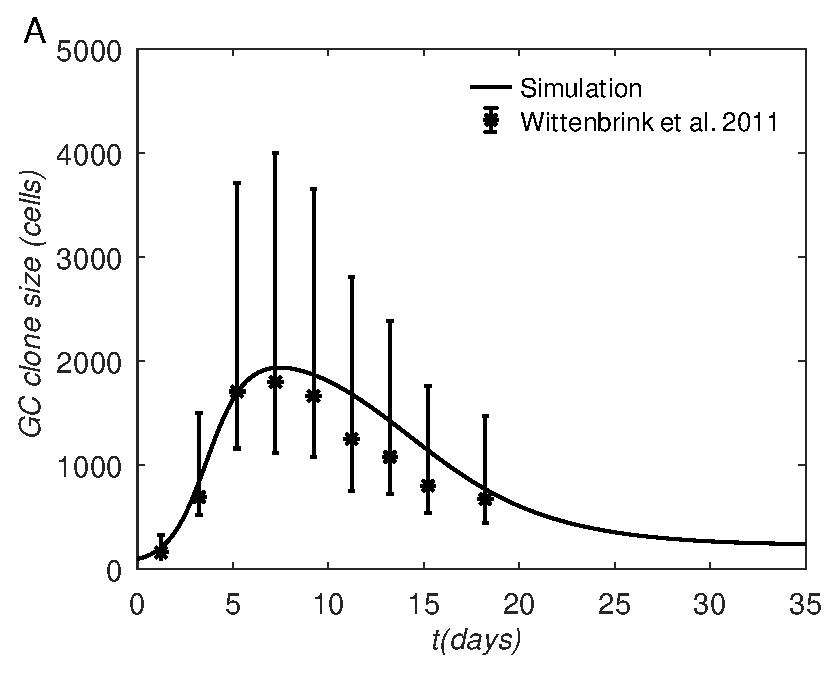
\includegraphics[width=0.32\textwidth]{../fig3/gcsize.eps}
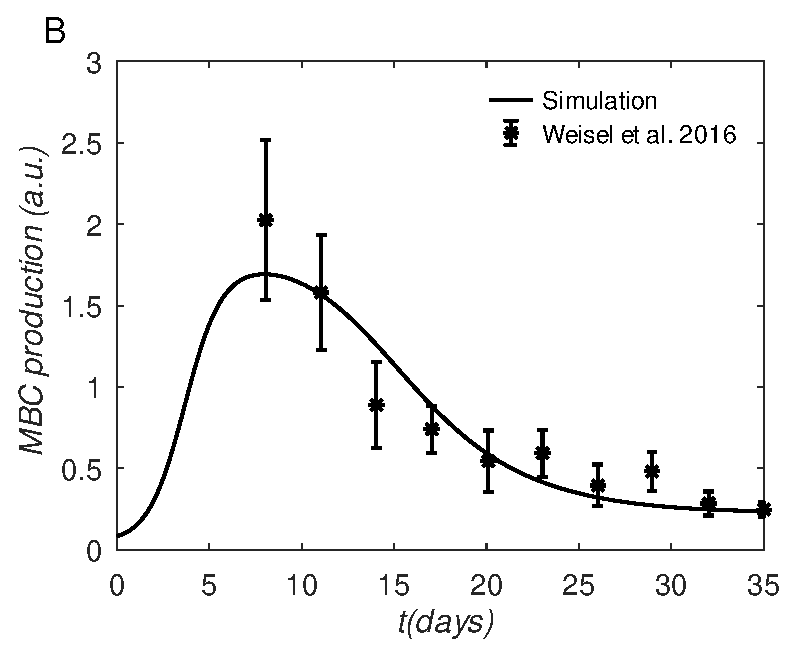
\includegraphics[width=0.32\textwidth]{../fig3/dmbc.eps}
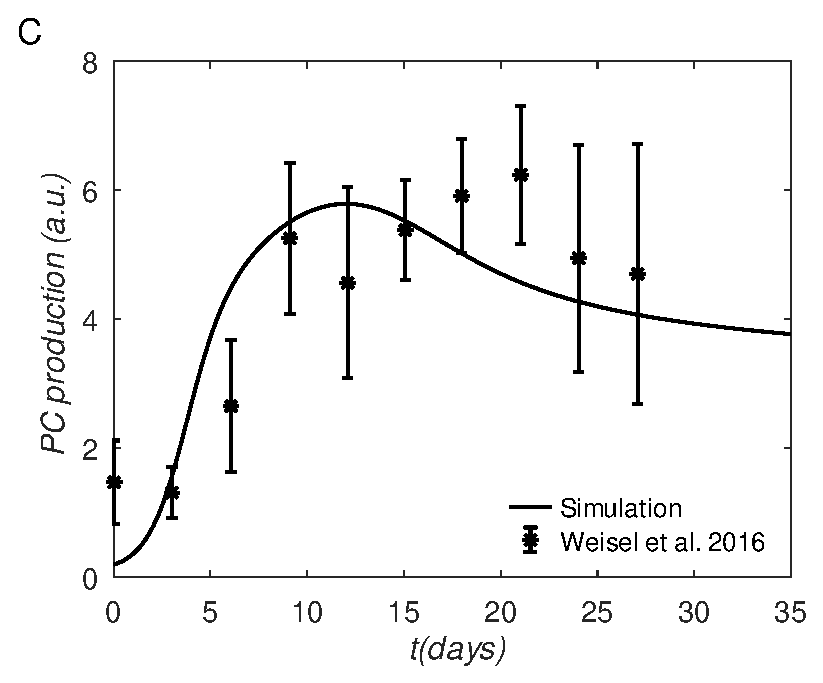
\includegraphics[width=0.32\textwidth]{../fig3/dplc.eps}
\caption{Comparison of simulation and experiments.
A: Total B-cells, B: Memory B-cell production rate, C: Plasma cell
production rate. Experimental data for panel A was generated from the GC
cross-sectional areas plotted in Fig.~S1B of Ref.~\citenum{wittenbrink11}, and converted to B cell counts
as done in Ref.~\citenum{pelissier20}; \vo{The lower and upper error bars in panel A
correspond to 30\%~and 70\%~quantiles, respectively};
experimental data for panels B \& C were taken from Fig.~4 of Ref.~\citenum{pelissier20}, who
obtained raw data from \citet{weisel16}; the error bars in B \& C correspond to approximately one SD, estimated from the 
range of the data, which we assumed to be Gaussian-distributed.
}
\label{fig:valid}
\end{figure*}
}

We first show that the model captures some experimentally determined
properties of GCs. In \fig{valid} we compare the model results obtained
with a single BCR/Ag pair to the average GC size reported by
\citet{wittenbrink11}, and the MBC and PC production rates determined by
\citet{weisel16}. The experimental data were also used by \citet{pelissier20}
to parametrize their stochastic GC model, which was used to explore the
mechanism of clonal bursts.
We note that the
\citet{wittenbrink11} observed very high CG size variability, as
reflected in the experimental error bars (\fig{valid}); thus, the
agreement between our model and the experimental average should be
considered as a qualitative validation, as the model does not capture GC size heterogeneity.

One apparent disagreement is that rate of PC production in our model is
accelerated by several days, compared to the data of \citet{weisel16}
(see \fig{valid}C).
\vo{Although the experimental MBC and PC production in \fig{valid}B \& C, respectively, correspond
to the same time, matching the PC production rate in the simulation required shifting the experimental
measurements by several days (compare \fig{valid}B with \fig{valid}C).}
%A possible explanation is that PC production occurs too rapidly in the simulations.
However, the discrepancy is not expected to affect our results
significantly, because we are interested in comparing the relative MBC
output from different lineages at the end of GC reactions, which are
simulated consistently, \ie~using the same model.

Next, we investigate the
effects of BCR binding avidity under different \vo{scenarios}. First, we compare the
growth rates of three noncompeting B-cell lineages, which differ only in
the value of the second-arm equilibrium binding constant $K^2_{eq}$ (written as $K^{i2}$ for lineage $i$ in \eq{binding} of Methods). This idealized
scenario corresponds to three GCs evolving independently, which is
the noninteracting, \vo{$\occl$=0, case (see Methods, \sec{occlusion}}), each completely dominated by a
single B-cell lineage. 

%For this simulation, and for several subsequent ones, 
We compare the behavior
of lineages with three regimes of bivalency, corresponding to $K^2_{eq}$=0,
$K^2_{eq}$=$K^1_{eq}$, and $K^2_{eq}$=10$K^1_{eq}$, which we denote,
respectively, as the monovalent, noncooperative, and cooperative binding
cases. The justification for the chosen values is discussed in the Methods \sec{avidity}.
%
\mk{[Would put in SI.]}\comment{moved to methods}
\hfig{
\begin{figure*}
\centering
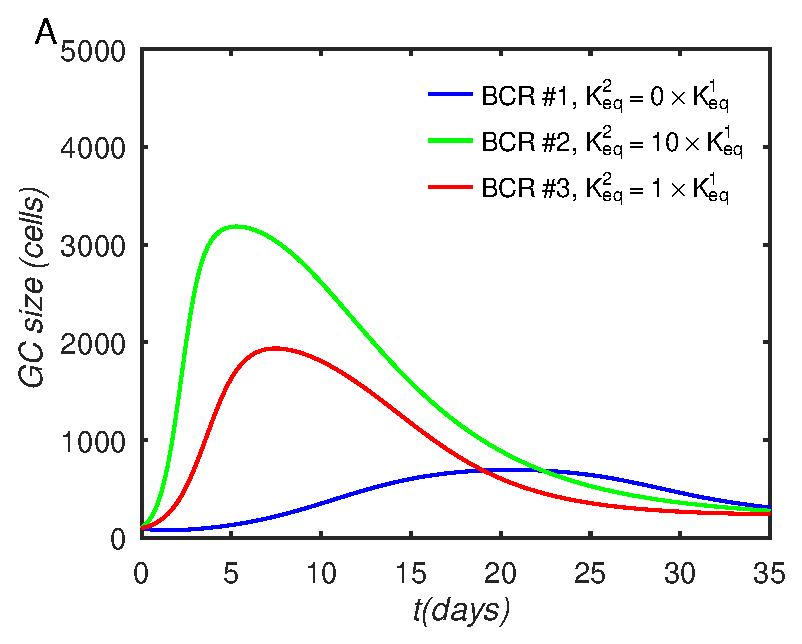
\includegraphics[width=0.49\textwidth]{../fig4abc/gcsize.eps}
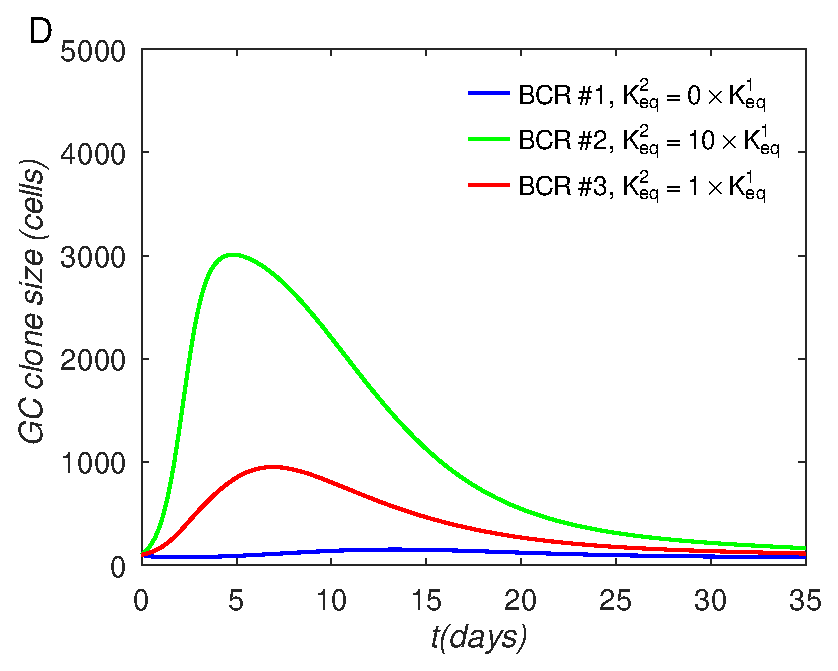
\includegraphics[width=0.49\textwidth]{../fig4def/gcsize.eps}
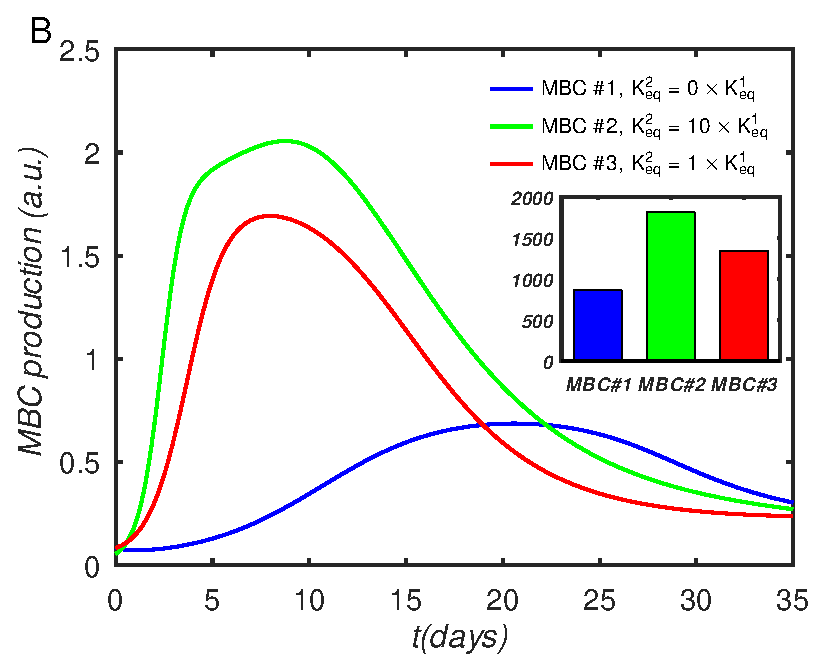
\includegraphics[width=0.49\textwidth]{../fig4abc/dmbc.eps}
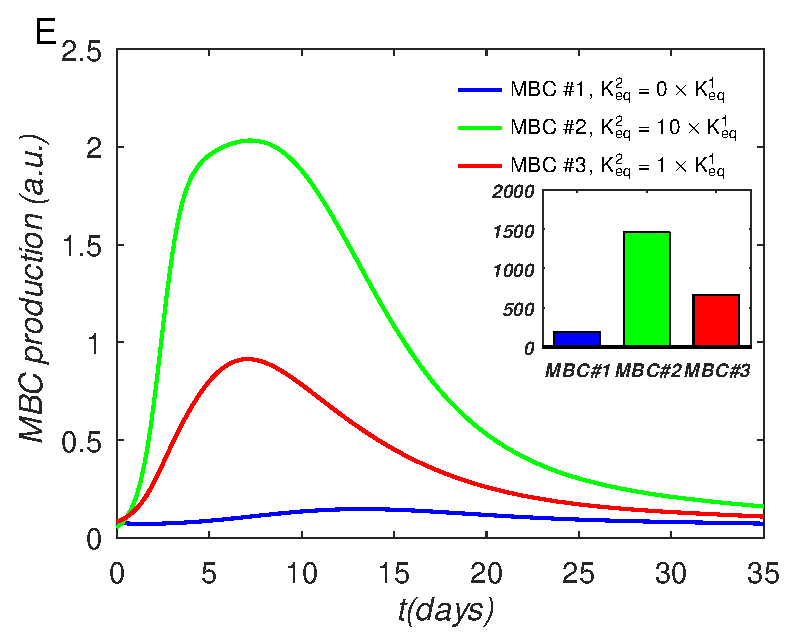
\includegraphics[width=0.49\textwidth]{../fig4def/dmbc.eps}
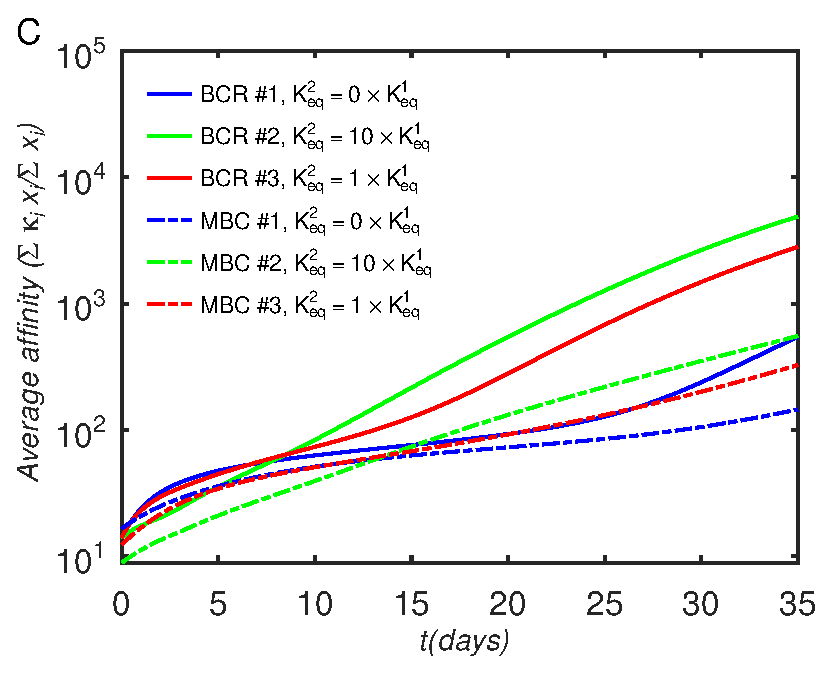
\includegraphics[width=0.49\textwidth]{../fig4abc/A.eps}
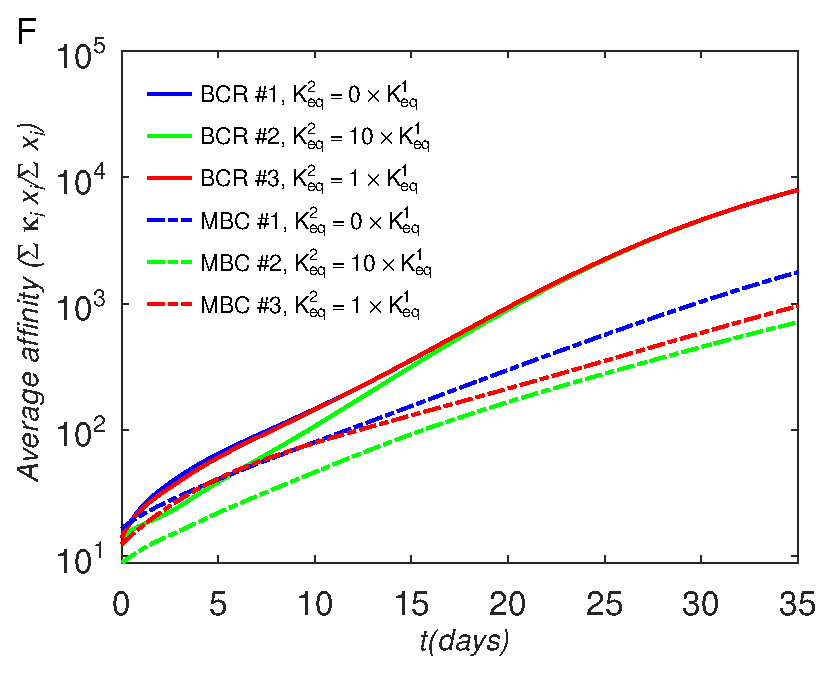
\includegraphics[width=0.49\textwidth]{../fig4def/A.eps}
\caption{Effect of antibody valency and epitope occlusion on GC properties.
Left column (A--C): noninteracting B-cell case ($o=0$);
Right column (D--F): fully interacting B-cell case ($o=1$);
A,D: Total B cells;
B,E: Memory cell production rate; insets: total MBC population at end of simulation;
C,F: Average affinity of B-cells and MBCs.  For the definition of occlusion $o$, see \sec{occlusion}.
}
\label{fig:avidity}
\end{figure*}
}

The results in \fig{avidity}A show that the monovalent BCR has a
significantly slower rate of growth compared with the bivalent BCRs, due to
the reduced activation by Ag assumed by the model. In the monovalent case,
the maximum B-cell count is less than a third of that in the bivalent
cooperative case, and less than half of that in the noncooperative case;
this lower maximum is also reached later; \ie, after 20 days, \vs~5 to 7 days.
Further,
the MBC count at the end of the GC is reduced by half in the monovalent case, compared with the cooperative case
(\fig{avidity}B), and the final average
affinity of the B-cell population is several-fold lower (\fig{avidity}C).
The delayed peak in the
monovalent response is qualitatively consistent with the observations of \citet{tan19},
who noted that the anti-influenza stem Ab response was delayed by a week relative
to the overall Ab response, and that the B-cell response was several-fold
lower in magnitude.

Although the noninteracting GC case is illustrative, it is idealized, because
in affinity maturation there will generally be many different B-cell
lineages competing for epitopes on the Ags, or for T-cell help
signals. Thus, a more realistic model of a single GC needs to account for
competition between different lineages. As described in \sec{occlusion} we
model this competition using an \textit{occlusion} parameter $\occl$, with $\occl=0$
for the fully noninteracting case, presented above, and $\occl=1$ for the fully interacting
(competing) case.
%
\cred{We note that a similar approach to model clonal competition was used by
\citet{Yan20}, who introduced interaction parameters to represent Ag
binding interference from Abs produced by earlier generations of B-cells.}

We describe the results of the fully interacting case ($\occl$=1) next; however, 
we note that a more realistic description of the overall GC reaction would probably
involve intermediate values of $o$. For example,
if, in some cases, different B-cells are able to bind to different epitopes
on the same Ag simultaneously, the occlusion parameter would need to be less than 1, which would
correspond to decreased competition between the B-cells. Moreover, when modeling
multiple GCs, it may be necessary to include the possibility that the Abs secreted by the plasma cells
can diffuse across many GCs, and compete with the `local' BCRs for
Ag.\cite{zhang13} This scenario would correspond to indirect
competition between different B cell lineages in different GCs, which might
be modeled with some optimized intermediate (though generally unknown) occlusion value.
\vo{A possible starting point for estimating such a value
could involve competitive binding experiments using antibodies specific for
the different epitopes.} 

The simulation of the fully interacting case shows that the
population disadvantage of the monovalent lineage is further increased
(\fig{avidity})D--F. The peak B-cell concentration of the monovalent lineage is more
than 10-fold lower than that of the bivalent cooperative lineage (panel D). These
results are to be expected, because the more rapidly proliferating lineage
occludes the Ag, effectively reducing the amount of epitope available to the
the monovalent lineage. The average monovalent MBC production is lower
by about a factor of \vo{eight} relative to the bivalent cooperative case (panel E).

It is noteworthy that the average affinities of the three BCRs are
indistinguishable after about 20 days after initiation of the GC reaction
in the fully competing case (panel F). Further, the BCR affinities in this
case at the end of the
simulation are higher than those in the $\occl$=0 case (\fig{avidity}C
\vs~\fig{avidity}F). This result is understandable in terms of increased
competition for survival inside the interacting ($\occl$=1) GC.  The fact
that binding by one BCR occludes access to other epitopes implies that
the effective epitope availability is decreased for all BCRs. 
A decrease in the available binding sites increases the
selection pressure on the BCRs, leading to the survival of the higher-affinity
lineages. We will return to this point when we investigate
the effects of varying epitope concentration explicitly. 
For completeness, simulation
results with intermediate values of occlusion are shown in Fig.~S1.

As discussed in the introduction, the reason for targeting immunosubdominant
epitopes such as the influenza HA stem or the interfacial
epitope\cite{watanabe19} in vaccinations is their association with the elicitation of bnAbs, which
are likely to provide protective immunity against future strains.
In the context of the present simulations,
such pre-existing protective immunity
can be modeled by increasing the initial affinity of the monovalent
antibodies, while keeping the other affinities unchanged.  This gives the
monovalent antibodies a survival advantage. A physiological
rationale of setting a higher initial affinity of monovalent Abs could
be that a significant proportion of monovalent (\eg, anti-HA stem) MBCs are recruted into secondary
GCs, where the higher initial affinity allows the MBC-derived blasts to compete more effectively with na\"ive bivalent B-cells.
%
\cred{A recent study comparing the early plasmablast (PB) response with GC
B cells obtained by fine-needle aspiration from vaccinated human subjects, found a variable, and sometimes large, clonal overlap
(12\% - 88\%) between B cells in the PB pool and those in the GC, suggesting that substantial 
recruitment of MBCs into GCs is possible.\cite{turner20}}
%
To model this scenario, we shifted the initial affinity distribution of the
monovalent Abs
%, which corresponds, as before, to lineage BCR\#1, 
by about two orders of magnitude towards higher values
(see the distributions in \fig{kadv}D), and repeated the simulations for the
fully interacting $\occl$=1 case (the $\occl$=0 case is shown in Fig.~S2).

\hfig{
\begin{figure*}
\centering
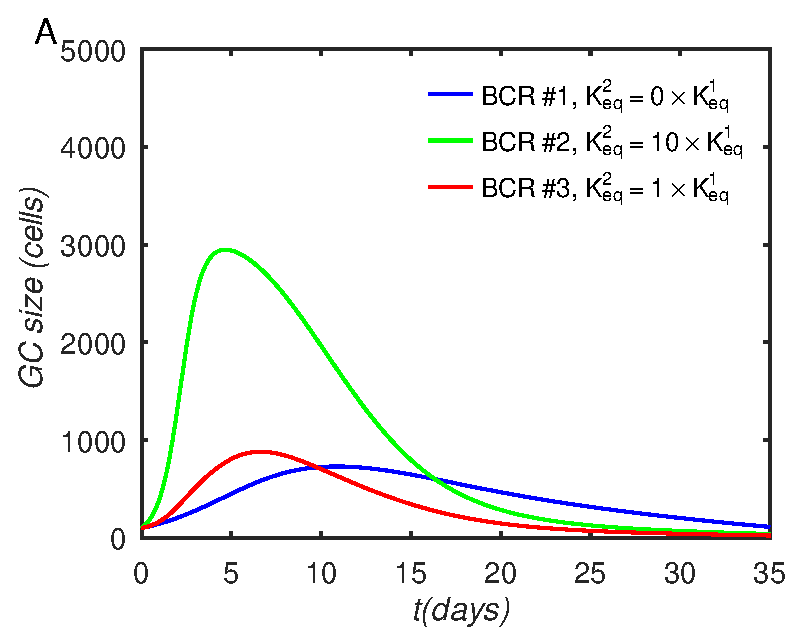
\includegraphics[width=0.5\textwidth]{../fig5/gcsize.eps}
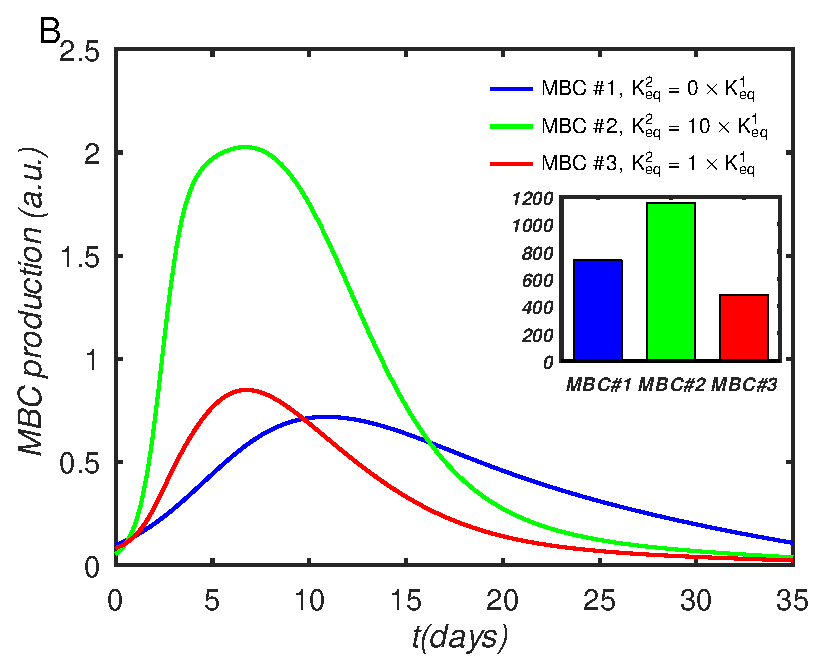
\includegraphics[width=0.49\textwidth]{../fig5/dmbc.eps}
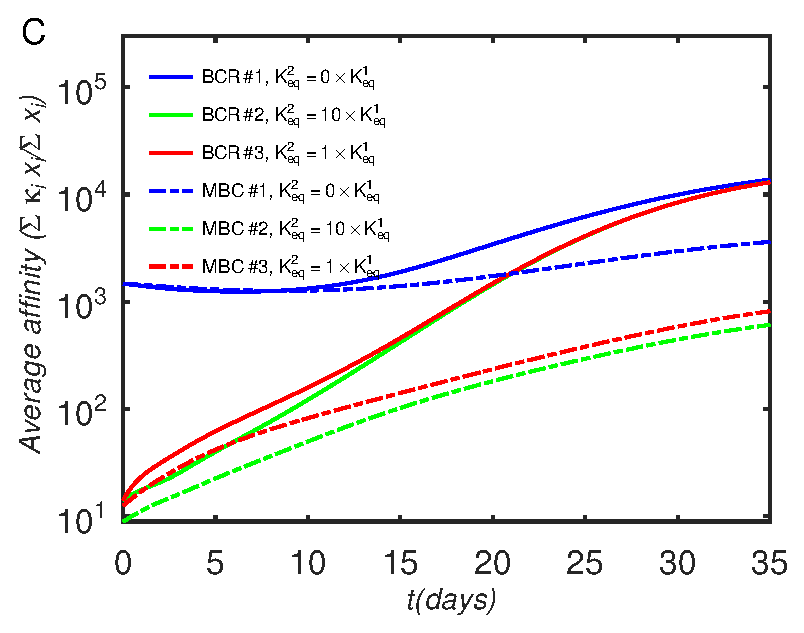
\includegraphics[width=0.5\textwidth]{../fig5/A.eps}
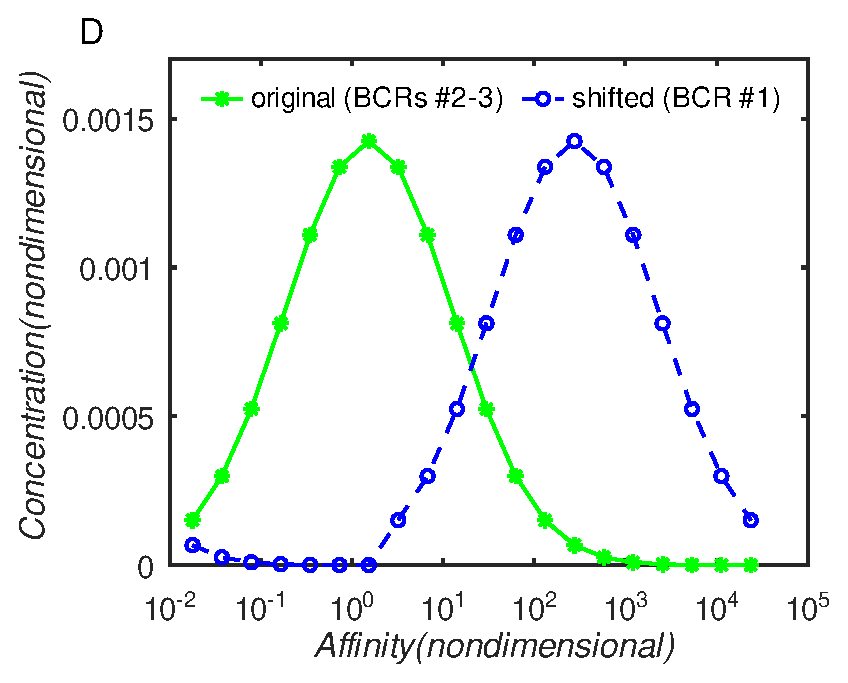
\includegraphics[width=0.49\textwidth]{../fig5/dist.eps}
\caption{Effect of initial affinity advantage on the growth of monovalent B-cells in the fully interacting B-cell case ($o=1$).
Panels A--C show the same quantities as \fig{avidity}A--C;
The affinity distribution corresponding to BCR\#1 was shifted toward higher values relative to BCR\#2 and BCR\#3
(panel D).
}
\label{fig:kadv}
\end{figure*}
}

\Fig{kadv}A shows that the population of the monovalent B-cells increased
several-fold as compared with \fig{avidity}D (no advantage),
such that, at their peak, these B-cells were almost as numerous as the bivalent
noncooperative ones. However, even the large affinity
advantage was insufficient to overcome the dominance of the
cooperatively-binding Abs in terms of the
total MBC response, which was still significantly lower in the monovalent
case (\fig{kadv}B).
\citet{nachbagauer17a} found that anti-HA stem immunity can be elicited or boosted upon immunization with
chimeric HA constructs with HA heads to which the host is na\"ive, fused to
HA stems against which there is preexisting immunity.
In other
studies,\cite{krammer12,ellebedy14} it was reported that boosting with
HAs from pandemic, rather than with seasonally-drifted strains, boosted
anti-stem immunity more effectively. The authors' interpretation of the results
was that the vaccinations boosted preferentially anti-stem responses derived from MBCs, which were
able to outcompete the na\"ive response to the HA head.
Further, \citet{ellebedy14} also found that immunosubdominance of the stem
reemerged after repeat immunization with the same pandemic strain.

To test whether the above findings could be explained with the present
model, we systematically repeated the preceding simulations for different
numbers of distinct BCR/epitope pairs (2 to 15), different occlusion
values $\occl$=[0,0.5,0.9,1], and three different values of affinity advantage provided to BCR\#1 (given below);
BCR\#1 bound monovalently ($K^{12}_{eq}$=0) or bivalently ($K^{12}_{eq}$=10$K^{11}_{eq}$).
The remaining BCR\#$i$ ($2\le i\le15$) were modeled as
bivalent with $K^{i2}_{eq}$=10$K^{11}_{eq}$. These simulations are discussed below, and their results are shown in \fig{kadv2}.

\vo{The goal of the simulations is to approximate conditions in which
one monovalent or bivalent anti-stem BCR (\#1) lineage is evolving concurrently with
1-14 bivalent anti-head BCRs.}
In the first vaccination, all BCRs start
from the same affinity distribution peaked at $K^1_{eq}\simeq$1.53 (\fig{kadv}D). To model
the effect of stem conservation after the first vaccination, BCR\#1 is
given a (multiplicative) affinity advantage over the remaining BCRs of $\Delta K_{eq}$=10, 100, or 1000.
After the first (prime) simulation, each boost is initialized with a
combination of 25\% MBCs taken at the end of the previous simulation,
and 75\% na\"ive B-cells having the same initial distribution as that used for the prime. We assume that
the previously-generated anti-head MBCs are poorly matched to the
boosting Ag and shift their affinity distribution toward lower values by
a factor of 1000, essentially eliminating any advantage of previous
maturation. For the presumptive stem-directed BCR\#1, we assume that the
previously-generated MBCs are better matched to the boosting Ag, and
shift their affinity downward only by a factor of 100, 10, or 1 (unchanged), to explore
the effect of the mismatch; (thus, the affinity advantage $\Delta K_{eq}$ of BCR\#1 corresponds to 1000
divided by 100, 10, or 1).
We found that the proportion MBC\#1 reaches a plateau by about
five immunizations (see Fig.~S3). In \fig{kadv2} we show the
fraction of MBCs\#1 after the sixth simulation.

\hfig{
\begin{figure*}
\centering
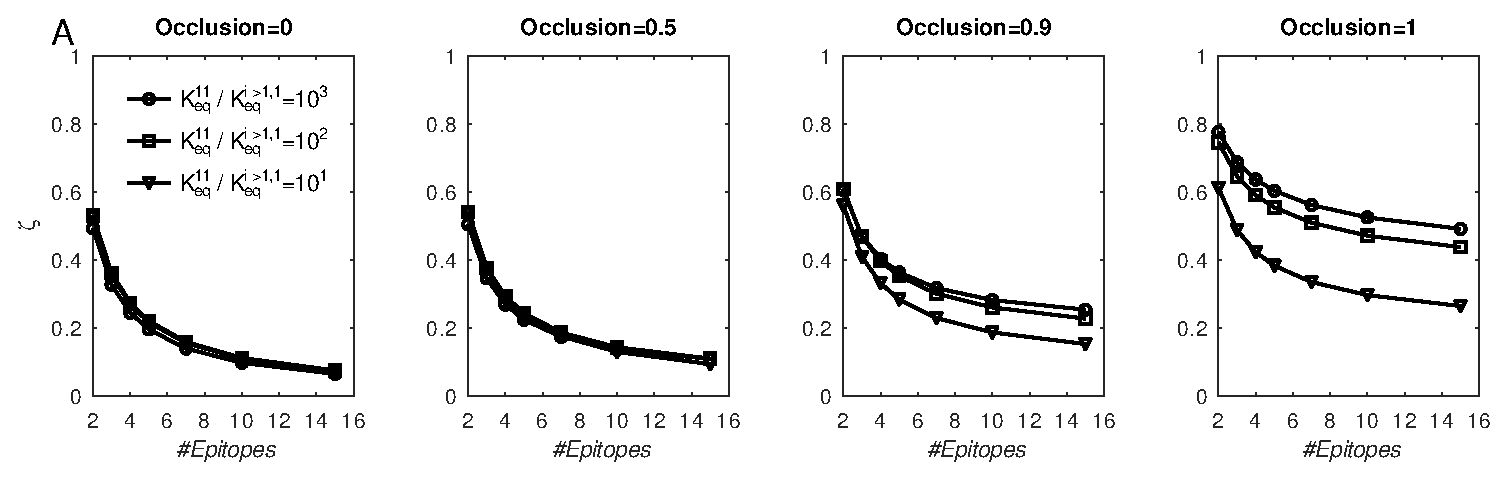
\includegraphics[width=0.99\textwidth]{../fig6/occl-k12=10agc1=1.eps}
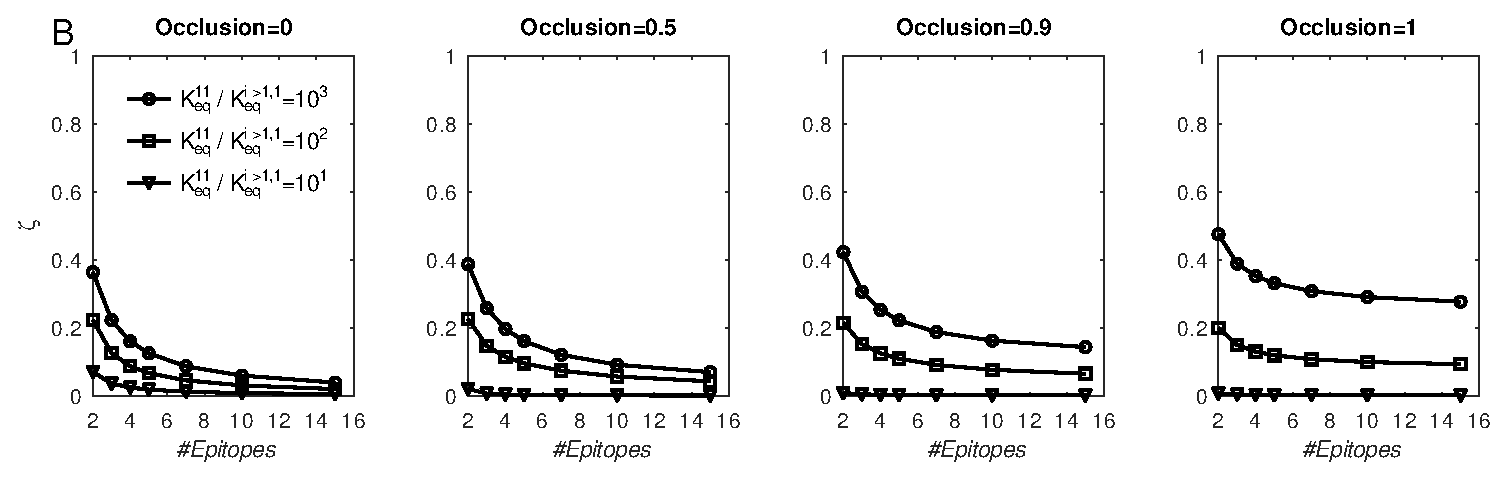
\includegraphics[width=0.99\textwidth]{../fig6/occl-k12=0agc1=1.eps}
\caption{Fraction of MBC\#1 ($\zeta$, \vo{defined in the text}) at the end of six GC simulations for different initial affinity advantage values
 \vs~total number of BCR/Epitope pairs.
A: BCR\#1 is cooperatively bivalent ($K^{12}_{eq}$=10$K^{11}_{eq}$);
B: BCR\#1 is monovalent ($K^{12}_{eq}$=0).
}
\label{fig:kadv2}
\end{figure*}
}
First, we discuss the results of the cooperative bivalent anti-stem case (\fig{kadv2}A).
Here, BCR\#1 does not have an avidity disadvantage (since it is cooperatively bivalent with $K^{12}_{eq}$=10$K^{11}_{eq}$),
relative to the
remaining BCRs, and has an affinity advantage, as described above. In the
noncompeting case ($\occl$=0) the MBC fraction
$\zeta$=$MBC_1/\sum_{i=1}^{N_B} MBC_i$ is not very sensitive to the affinity
advantage, because the Abs are maturing independently and the
concentration of each epitope is the same. As the competition between
the BCR lineages is increased, the affinity advantage becomes more
important. For example, in the high occlusion cases $\occl\ge 0.9$, with 9
competing low-affinity BCRs, a 1 to 3 order of magnitude affinity advantage results
in $\sim$20\% to $\sim$50\% of the final MBC population being derived from BCR\#1
\vo{($\zeta\in[0.2,0.5]$ in the two right panels of \fig{kadv2}A).}

In contrast, the monovalent anti-stem response (\fig{kadv2}B) produces
markedly lower, though still significant MBC\#1 proportions. For the
lowest initial affinity advantage ($\times 10$), the proportion of MBC\#1 is
vanishingly small for all interacting cases. For the higher advantage values
($\times 100$ and $\times 1000$), the proportion of MBC\#1 with 9 competing low-affinity
BCRs at $\occl\ge 0.9$ is in the range $\sim$10\% -- $\sim$30\%
\vo{($\zeta\in[0.1,0.3]$ in the two right panels of \fig{kadv2}B).}

We interpret these results to suggest that a previous response to a conserved
epitope could be boosted to dominate the subsequent response, even in the
presence of a significant number of poorly-conserved `distracting'
epitopes.  This is consistent with the chimeric vaccination results of
\citet{nachbagauer17a}. However, the extent of boosting is
critically dependent on the affinity advantage of the preexisting
immunity. In the case of monovalent antibodies, the affinity
advantage needs to be high to \vo{overcome} the proliferation
disadvantage caused by monovalency, and the entropic disadvantage
caused by distracting epitopes that generally outnumber conserved ones.
\citet{ellebedy14} noted that vaccination with a pandemic strain against
which anti-HA head immunity is low, preferentially boosted anti-HA stem
antibodies. However, upon reimmunization with the same antigen, the
anti-HA head Abs were boosted preferentially. These results can be
rationalized in the present model by the
differential affinity advantages of the anti-HA stem Abs.  Specifically, for the first
immunization, the anti-stem immunity has a sufficient affinity advantage
to overcome the growth-related and entropic disadvantages. For the second
immunization, the affinity advantage is eroded because the anti-HA head
immunity has undergone affinity maturation caused by the first
immunization, which leads to the restoration of stem epitope
subdominance.

Because the affinity advantage of a conserved epitope cannot be predicted
accurately if antigenic drift is present, a more realistic approach would
be to treat $\Delta K_{eq}$ as a random variable. To investigate this
scenario, we performed a round of simulations in which $\Delta K_{eq}$
was sampled from the lognormal distribution; the results are described in
\SI~S1. The differences between the
two cases were similar to those in the simulations with
fixed $\Delta K_{eq}$. For example, in the bivalent case, some MBC\#1
cells were always present, while in some simulations of the
monovalent case the MBC\#1 proportion is near zero (see Fig.~S4).

The above simulations suggest that an affinity advantage alone will not always be
sufficient to overcome the disadvantage of slower proliferation and
entropic distraction. This result, together with other factors, such as low
germline precursor frequency or T-cell help insufficiency,\cite{tan19}
could explain the lower prevalence of anti-HA stem immunity.

In natural infections, the epitope concentrations are predetermined by the Ag itself (\eg,
the solvent-accessible surface area of the HA head on an influenza virion
is about twice that of the stem; see Fig.~S5 in \SI~S2).
%
However, the vaccination setting allows use of designed antigens with
some epitopes masked by glycosylation\cite{bajic19,eggink14,zhou17} or
even completely removed using protein engineering\cite{yassine15,corbett19}. Additionally, one can
administer concurrently multiple Ags, in which some Ag epitopes are
sufficiently conserved between the antigens that they can be considered
to represent a single epitope with a higher effective concentration.
\cite{kanekiyo19,Boyoglu-Barnum20,cohen21,glanville20}.
In the next set of simulations, we investigate the interplay of epitope
concentration and BCR binding valency.
%
\hfig{
\begin{figure}
\centering
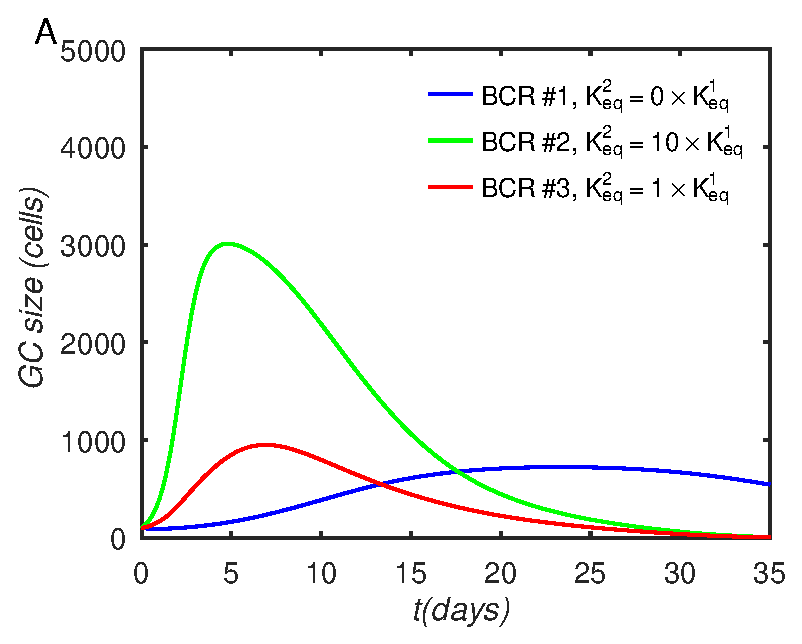
\includegraphics[width=0.49\textwidth]{../fig7/gcsize.eps}
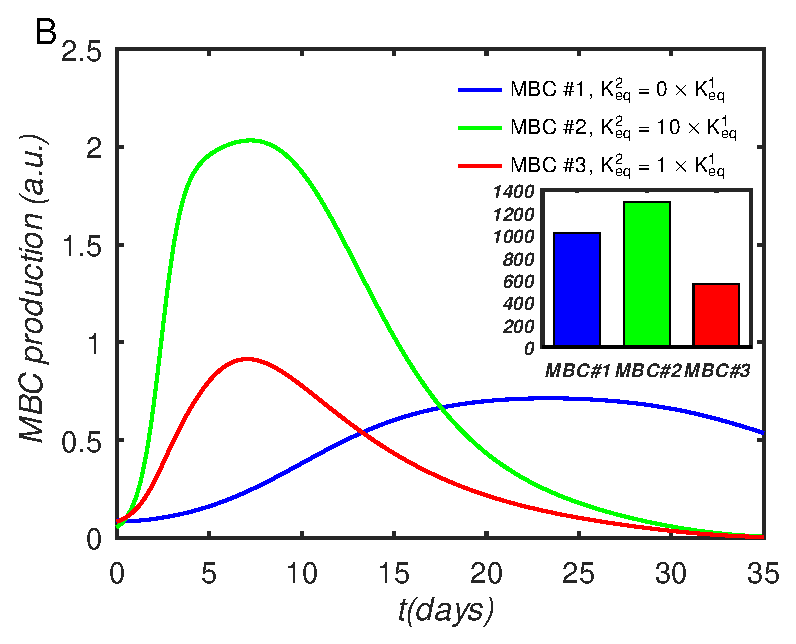
\includegraphics[width=0.49\textwidth]{../fig7/dmbc.eps}
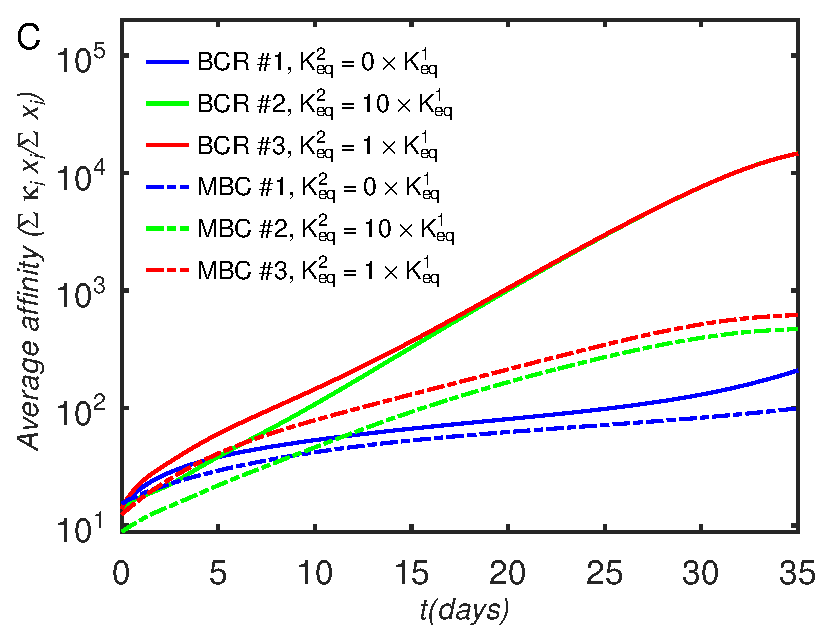
\includegraphics[width=0.49\textwidth]{../fig7/A.eps}
\caption{Effect of BCR valency and epitope concentration on GC evolution, with $o=1$ (fully competitive case).
Panels A--C show the same quantities as \fig{avidity}A--C;
$\alpha_1^T=2$, $\alpha_2^T=1$, $\alpha_3^T=1$; $\alpha^T$ is the nondimensional total Ag concentration (see \sec{integration}).
}
\label{fig:agc1}
\end{figure}
}
%
\Fig{agc1} shows the results of a GC simulation involving three
competing BCR/Ag pairs, for comparison with the previous 3-BCR simulations (\figs{avidity}{kadv});
the noninteracting case can be found in Fig.~S6.
The concentration of
Ag\#1, which corresponds to the monovalent BCR\#1, was twice that of
the other two Ags, while all other parameters were the same as in the
original 3-BCR simulation. The peak monovalent
B-cell population increases several-fold relative to the uniform concentration
case (\fig{avidity}D); it is similar in magnitude to that in the
affinity-advantaged case of \fig{kadv}, but occurs later, at $\sim$23 \vs~$\sim$11 days. This
behavior was expected, because, although BCR\#1 has an impaired
growth rate due to monovalency, it also has more antigen available, allowing it
to grow for longer times. Even though the other (bivalent) BCRs are
occluding, the higher concentration of Ag\#1 overcomes the occlusion disadvantage,
albeit with a slow growth rate. The resulting MBC\#1 population
is much closer to that of the bivalent cooperative case.
However, although the greater abundance of Ag\#1 amplifies the total BCR\#1
response, it also reduces the competition for this Ag, which results in
a lower overall affinity of the resulting B-cells (\fig{agc1}C).

For completeness, in \SI~S3 we repeated the above simulation while systematically varying the
number of BCR/epitope pairs \vo{(2-15)}, occlusion parameter value \vo{(0,0.5,0.9,1)}, with
three values of affinity advantage provided to the
BCR\#1, and with the BCR\#1s bound monovalently or bivalently. The results are summarized in Fig.~S7.
In all cases, increasing Ag concentration leads to
greater MBC output, with the increase being larger if the
corresponding BCR also has a significant affinity advantage.
The increased MBC output is associated with decreased affinity, however, and the affinity decrease
is larger for monovalent than bivalent
BCR\#1s. The results therefore suggest that
epitope subdominance can be overcome by increasing epitope concentration
in vaccinations with cocktails of designed antigens, as proposed by
others.\cite{kanekiyo19,cohen21,glanville20}  However, this is \vo{achieved} at the expense of a
reduction in the affinity of the resulting MBCs.
For vaccine design, the precise Ag concentrations may need to be 
optimized to achieve a compromise between MBC population
size and affinity for antigen.

\cred{
We caution, however, that the above results should be considered qualitative,
because our model does not incorporate a saturating Ag concentration, which could be done 
in fugure versions, \eg, by explicitly modeling immune complexes or FDCs.
Thus, the strong dependence of B-cell response on the Ag concentration
is most likely relevant in a scenario where the total antigen amount is low.
}

Finally, to investigate whether the outcome of multiple vaccinations can
be optimized by manipulating the epitope concentrations corresponding
to monovalent BCRs, we simulated six consecutive immunizations under the
same initial conditions as described before, except that the
concentration of Ag\#1 was increased in some, but not all, of the simulations.
Specifically, we considered three immunization scenarios, in which the total nondimensional concentration of Ag\#1,
$\alpha^T_1$=[Ag\#1/Ag\#i$>$1], in the six consecutive immunizations was
(1, 1, 1, 1, 1, 1), (2, 1, 1, 2, 1, 1), and (2, 2, 1.5, 1.1, 1, 1). These
three scenarios were chosen to determine whether increased Ag\#1
occurring early in a vaccination regimen would translate into superior
responses in later exposures.
%
\hfig{
\begin{figure*}
\centering
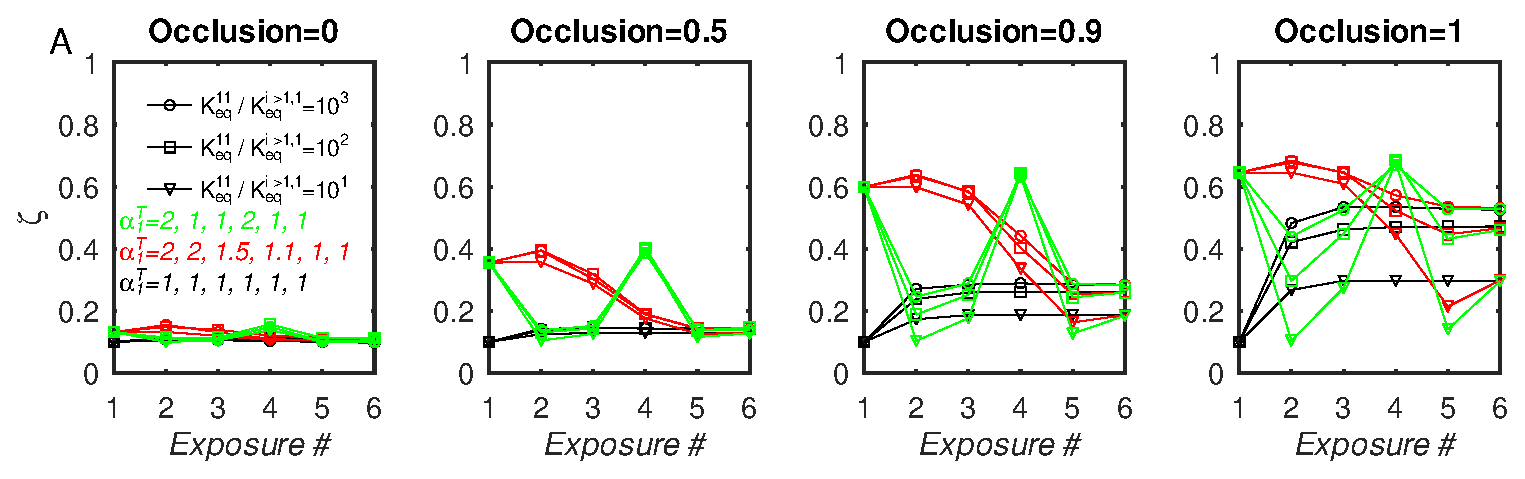
\includegraphics[width=0.99\textwidth]{../fig8-S3-S8/mbctime-k12=10.eps}
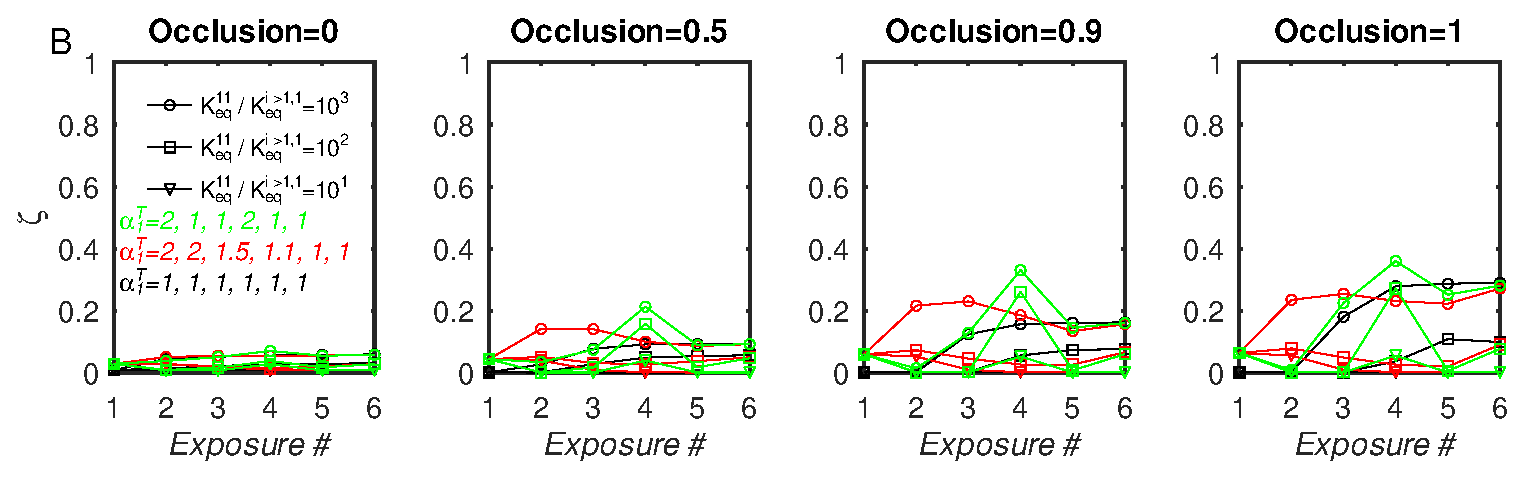
\includegraphics[width=0.99\textwidth]{../fig8-S3-S8/mbctime-k12=0.eps}
\caption{Fraction of MBC\#1 \vs~number of sequential GC simulations for different initial affinity advantage values
and different Ag\#1 concentrations, with 10 total BCR/Epitope pairs.
A \& B: MBC\#1 fraction ($\zeta$) at the end of simulations.
A: BCR\#1 is cooperatively bivalent ($K^{12}_{eq}$=10$K^{11}_{eq}$);
B: BCR\#1 is monovalent ($K^{12}_{eq}$=0).  
The four sets of panels A and B show the effect of increasing occlusion from $o$=0 (no
competition) to $o$=1 (full competition).
}
\label{fig:agtime}
\end{figure*}
}
%\Figs{agtime}{agtime2} show the MBC output and affinity at the end of each
Figures~\ref{fig:agtime} and S8 show the MBC output and affinity, respectively, at the end of each
immunization for ten BCR/epitope pairs (other cases are omitted for
clarity, but are qualitatively similar). Consistent with the previous
results, MBC\#1 output after a particular immunization increases if
Ag\#1 used in that immunization is increased (and vice versa), and the
MBC\#1 affinity decreases if Ag\#1 used in that immunization is increased
(and vice versa). However, the differences between the three protocols
essentially disappear after the final exposure, hence the present model suggests that there
may not be a significant long term immunological effect of simply
manipulating antigen concentration in a vaccine.

\cred{We also note that, in the idealized case of a uniform antigen concentration
profile, the normalized BCR affinities for antigen rise uniformly to a
plateau around the 5th exposure (Fig.~S8). However, the results show a
sensitivity to the antigen concentration profile, suggesting that the
number of exposures needed to elicit high-affinity antibodies generally
depends on the details of the exposure, such as epitope concentration, or
whether the exposure is by vaccination or natural infection.}

\section{Discussion}
\label{sec:discussion}
Rapidly mutating and proliferating viruses such as influenza, HIV, and,
more recently, SARS-CoV-2, accumulate escape mutations that can
render existing host immunity obsolete. However, because such pathogens
must maintain infectivity to survive, some mutations are highly
improbable, as they would significantly reduce or even eliminate viral
fitness. In addition, selection pressure from the immune system is variable
along the antigenic sequence (\eg~solvent-exposed regions are more susceptible to antibodies than buried ones).
The resulting differences in mutation
propensities make it possible to partition the viral topology into variable and conserved epitopes.
Unfortunately, variable epitopes tend to be immunodominant, \ie~they are the main
targets of adaptive immunity. Immunodominance, in itself, may be the result of viral
adaptation; for example, the large highly-variable head of influenza hemagglutinins
is an entropic distraction to the immune system.
A major focus of current vaccine research is to elicit a potent and durable
immunity to conserved, immunosubdominant, epitopes.  Such vaccines
would
lower HIV infection rates, or eliminate the need for a yearly influenza
vaccine.

Here, we employed a coarse-grained model of affinity maturation (AM)
parametrized using experimental data on germinal centers
(GCs)\cite{wittenbrink11,weisel16,pelissier20} to determine whether
differences in B-cell receptor (BCR) binding valency could explain the
subdominance of certain epitopes. The main assumption of the model is
that B-cell activation increases with the amount of equilibrium-bound BCR
to antigen (Ag). More specifically, when both arms (Fabs) of BCR bind the antigen
displayed on follicular dendritic cells (FDCs), the probability of
internalizing the Ag increases, even if the affinity of each
receptor for Ag is weak. This assumption appears to be in accord with the
experiments;
\citet{arevalo20} interpreted their vaccination boosting data by
suggesting that many weak BCR/Ag interactions are sufficient to activate
B-cells. Compelling indirect evidence comes from co-display of
different Ags on nanoparticles, which was \comment{referring to co-display, which is singular} demonstrated to preferentially
elicit broadly-neutralizing Abs.  These findings\cite{kanekiyo19,cohen21}
imply that avid bivalent binding confers a proliferation advantage,
which is consistent with the present model. However, as B-cell activation by
Ags is
a complicated process, involving cross-linking of the BCRs, it is not
clear to what extent avid binding would increase crosslinking.
Future experiments and simulations may be needed to shed more light on the activation
process.

The present simulations indicate that monovalent B-cells always
grow more slowly than bivalent ones, and are therefore easily dominated by B cells that are able to bind bivalently and
cooperatively. When given an initial affinity advantage over bivalent
B-cells, as might be expected to occur upon recruitment of monovalent memory
cells (MBCs) into secondary GCs, the affinity advantage was often
insufficient to overcome the slower growth.
The monovalent B cells outcompeted bivalent ones only if the
affinity advantage was more than an order of magnitude (see \fig{kadv2}B). These
results are in agreement with influenza vaccination experiments, which show
that a boost with a pandemic strain for which the host has little
immunity against epitopes in the HA head, produces high anti-HA stem
titers; a subsequent boost with the same vaccine elicits anti-HA head
Abs.\cite{ellebedy14} We have interpreted these experimental data by assuming 
that anti-HA stem Abs bind monovalently with
a high affinity advantage in the first vaccination, but not the second.
In the second vaccination, the bivalent anti-HA head 
Abs are able to overcome the advantage \via~maturation induced by the first shot.

Rather than relying solely on an affinity advantage, a more robust method
to boost monovalent B-cells is to increase the concentration of their cognate
epitope(s). The simulations indicate that this approach results in the highest
number of monovalent MBCs (see \figs{agc1}{agtime} in \sec{results}).
The finding is not surprising, since the presence of foreign
antigen is what initiates and sustains GC reactions in the first place.
However, because selection among B-cells is driven by competition for Ag, an
increase in available Ag will allow lower-affinity BCRs to survive.
Thus, although the corresponding monovalent Abs become more numerous with increased epitope concentration,
they evolve lower average affinity.
When we simulated a subsequent
GC reaction initialized with MBCs from such a memory pool, but
\textit{without} the concentration advantage (designated by $\alpha_1^T=1$ in
the results), as would occur in a
natural infection, the monovalent B-cell population rapidly decreased,
such that after two such consecutive GC reactions, there was no difference
when compared to vaccinations in which the concentration of the Ag
cognate to the monovalent Ab was never increased (\fig{agtime}).

These results suggest
that increasing Ag concentration might only provide a temporary advantage
to the cognate BCRs, as Ag levels are easy to manipulate in
vaccination, but not in infection. \cred{Nevertheless, the strategy could prove
useful to expand the number of initial low-affinity B-cell lineages
targeting rare epitopes against which high-quality B-cell precursors are
rare, such as group I and II influenza stem epitopes, as also suggested 
in a recent computational study of COVID vaccine efficacy.\cite{garg21}}

If subsequent
exposures \via~natural infection restore immunosubdominance,\cite{ellebedy14} regular
vaccine boosting with higher concentrations of subdominant epitopes could be
required.


\cred{We note that multi-antigen vaccination cocktails have been designed, in
which the epitopes that are conserved between the antigens are at
effectively higher concentration than variable
epitopes.\cite{kanekiyo19,cohen21,glanville20} In particular, mosaic
nanoparticles appear to elicit a broader antibody response in animal
experiments, compared to cocktail immunizations.\cite{kanekiyo19,cohen21}
However, it remains to be shown whether such vaccines will lead to
improved protection against highly mutable pathogens in the clinic.}
%
Simulations performed here suggest that such cocktails have promise to
elicit Abs to conserved epitopes \via~a concentration advantage.  Future
experiments are needed to address whether the resulting immunity would
persist after multiple rounds of natural infections.

The model used here relies on simple assumptions to show that for different
epitopes with similar accessibilities, which can be interpreted as
similar effective concentrations, immunosubdominance can be explained by
differences in the antibody binding valency. This scenario appears
applicable to the case of  natural immunity against influenza
hemagglutinins, as \citet{harris13} have shown that most of the trimeric
HA spikes are able to bind an anti-stem antibody. The arrangement of the
spikes makes it likely that bivalent binding would be disfavored by energetic
strain.\cite{harris13,amitai20} A related scanario applies in the
case of HIV, in which low spike density makes bivalent binding unlikely,
but antibodies engineered with long linkers  that could bind the same
trimeric spike bivalently exhibited $>100$-fold greated potency.\cite{galimidi15}
%
\cred{
However, binding valency alone cannot adequately explain immunodominance 
that arises in vaccination using soluble HA ectodomains, because
head and stem epitopes would be expected to have similar antibody accessibilities.
Therefore, other factors, such as antigen plasticity, low natural germline
precursor frequency, repertoire filtering due to self-reactivity, or
reduced T-cell help,\cite{erwin20} must also contribute.
}
%
\cred{For example, \citet{keating20} employed several methods of partially inhibiting GC
formation in mice, and showed that the proportion of bnAbs in GC-inhibited
mice was not increased relative to wild-type mice or untreated mice. The
findings were used to argue that the predominant reason for low bnAb
prevalence was not competition between antibody lineages, but other
factors, such as removal of bnAb precursors due to immune tolerance
mechanisms.\cite{keating20} Such factors could also explain
why antibodies produced in natural infections such as SARS-Cov-2 tend to target relatively
few antigenic epitopes, despite high overall antigen accessibility.\cite{barnes20}}

Some of the aforementioned factors could be incorporated into the model
in an approximate way in future studies.
%
\cred{The effects of adjuvants on B-cell activation can be modeled by
parametrizing the B-cell activation function to include
adjuvant concentration, or by incorporating the latter into a T helper cell model.
Similar ideas could be used to include the effects of soluble signaling
species, such as interleukins or Calcium ions.}
%
\cred{Further, more sophisticated approaches that explicitly model BCR evolution in
sequence space and/or compute BCR/Ag binding affinity using structural models have been developed.
For example, \citet{robert21}
approximated B-cell and Antigen interactions by discretizing the epitope
and paratope on a lattice, and using an empirical inter-residue
potential.\cite{robert21} The authors were able to capture key properties 
of multi-antigen vaccinations, such as increased cross-reactivity in
cocktail immunizations.}
%
\cred{
However, BCR/Ag models at all-atom resolution,\cite{conti21,sprenger21}
which may be parametrized to account for antigen stability and rigidity,
may ultimately be required to design actual vaccine antigens and their
cocktails.
}

\cred{For the practical purpose of universal vaccine
design, we can summarize the interpretation of our simulation results as
follows.  HA stem epitopes presented on influenza virions are
immuno-subdominant due to an inability to recruit bivalently-binding
BCRs, combined other causes of subdominance. Even if vaccination with
soluble antigen ectodomains elicited an anti-stem response, it would not
be boosted in secondary GCs formed upon subsequent natural reinfection, 
because the corresponding B-cells would be unable to bind antigen
bivalently. It remains to be shown whether this disadvantage could be
overcome by devising vaccines that present stem epitopes for bivalent
binding, \eg~by using engineered immunogens attached to
nanoparticles,\cite{corbett19} possibly in a mosaic
arrangement\cite{cohen21}, or by immunizing with cocktails with very
similar stems but diverse heads\cite{glanville20}.}

\cred{While
immunization with diverse coronavirus receptor binding domains presented
as mosaic nanoparticles elicited a broad antibody response, including to
strains not present in the vaccine,\cite{cohen21} when this strategy was
applied to a diverse panel of influenza HA spikes, the resulting breadth
was no greater than that observed with immunizations using homotypic
nanoparticle cocktails.\cite{cohen21a} The interpretation was that the
epitopes in the mosaic panel were too dissimilar to allow significant
bivalent binding, which suggests that careful tuning of antigen sequence
similarity may be needed to elicit broad responses \via a concentration
advantage.}

\section{Methods}
\label{sec:methods}

\subsection*{Model of Germinal Center Affinity Maturation}

The model of affinity maturation (AM) used here is based on the work of
\citet{kepler93},
who used systems of coupled
differential equations to calculate the concentrations of B-cells of
different discrete affinities for an antigen (Ag). %, with fixed total Ag concentration.
We have generalized the model to
simulate the maturation of multiple B-cell lineages, each binding to its cognate
antigen mono- or bivalently, and producing memory B-cells and plasma
cells, which secrete antibodies of the same affinity for the cognate Ag. The model does not have any
geometric or topological component to represent binding, and, where there is no ambiguity, we sometimes use
the terms antigen and epitope interchangeably. We will also sometimes use
the abbreviation BCR (B-cell receptor) to refer to B-cells, with the implicit
scaling assumption that each B-cell has $\sim10^5$ BCRs on its surface.\cite{casten88,Alberts02}

We assume that the simulated germinal center(s) (GCs) have been seeded by
$N_B$ B-cell lineages $B^i$, and that each lineage can bind only to its cognate
antigen $a_i$. Though the model is based on the system of differential equations
of \citet{kepler93}, it has several important additions, \vo{notably}
memory cell, plasma cell, and antibody production. For clarity, we first present
a minimal version of the model, which is close to the original B-cell model\cite{kepler93} and describe the modifications in
subsequent subsections.
\hide{A visual schematic of the model components was given in \fig{model}.}
\subsubsection{Basic model}
\label{sec:basic}
For each B-cell lineage, we explicitly
model its binding affinity distribution. Specifically, we
assume that (1) the equilibrium binding affinity $K_{eq}^i$ of any B-cell $B^i$ derived from the lineage $i$
for its cognate antigen $a_i$ is in the range $K_{eq}^{min}\le K_{eq}^i \le K_{eq}^{max}$ and (2) that the affinities
can be represented by a discrete set of values, as follows. We assign to each $B^i$ a binding energy index $j\ge1$ such that
\begin{equation}
 \begin{aligned}
% \log K^{min}_{eq}\le& (j-1)\Delta E+\log K^{min}_{eq}\le \log K_{eq}^i \\
%               <& j\Delta E + \log K^{min}_{eq}\le\log K^{max}_{eq} +\Delta E.
 \log K^{min}_{eq}\le& (j-1)\Delta E+\log K^{min}_{eq}\le \log K_{eq}^i
               < j\Delta E + \log K^{min}_{eq}\le\log K^{max}_{eq} +\Delta E.
 \end{aligned}
 \label{eq:grid}
\end{equation}
\Eq{grid} corresponds to a uniform discretization of binding
affinities in logarithmic space with energy grid spacing $\Delta E$, or exponential
discretization in affinity space.

As done by \citet{kepler93}, we will refer to the energy bins $j$ as
\textit{affinity classes}. Their number, $N_\epsilon$, is related to $\Delta E$ by $\log K^{max}_{eq} - \log K^{min}_{eq} =
(N_\epsilon-1)\Delta E$. We take
$N_\epsilon$=20 (see \tab{param}), which implicitly determines $\Delta E$
once $K^{min}_{eq}$ and $K^{max}_{eq}$ are chosen. In the simulations, we only
allow values of $K_{eq}$ that correspond to the bin edges, \ie,
$K^i_j=K^{min}_{eq}e^{(j-1)\Delta E}$, $1\le j\le N_\epsilon$, where,
for brevity, we replaced the subscript $eq$ by the affinity class index $j$.

To simulate affinity maturation, we compute the time evolution of B-cell
populations in each affinity class $j$ using \mk{Should the second term in the
first brackets by ``$+k_p$''?}\comment{No, can compare with Kepler93 ref.}
\begin{equation}
\begin{aligned}
 \td{[B^i_j]}{t}=&\left\{-k_d(1-h^i_j) - k_p\right\}[B^i_j] + 2k_p\sum^{N_\epsilon}_{k=1} m_{kj} [B^i_k],\\
  \textrm{for}\ 1\le& i\le N_B,
\end{aligned}
 \label{eq:am}
\end{equation}
where $k_p$ and $k_d$ are proliferation and death constants, respectively, $m_{kj}$ is the probability
for a BCR $B^i$ in affinity class $k$ to transition to affinity class $j$ \via~somatic mutations that take place during AM,
$h^i_j$ is B-cell activation function (discussed below), and $N_B$ is the number of different B-cell lineages.

The class transition probabilities $m_{jk}$ are assumed to be independent of the lineage $i$, and are defined as
\begin{equation}
 \begin{aligned}
  &m_{jk}=\frac{\left[\mu(1-p_L)\right]^{\snorm{k-j}}}{\snorm{k-j}!} \frac{\exp(-\mu)}{1+\Lambda^{2(k-j)}}, \quad j\ne k \\
  &m_{jj}=1-\sum_{k\ne j}^{N_\epsilon} m_{jk},
 \end{aligned}
\end{equation}
where $\Lambda$ \vo{determines} the ratio of advantageous to non-lethal deleterious mutations, $p_L$ is the probability of lethal mutations,
and $\mu$ is the probability of an expressed (\ie~nonsilent) mutation per generation.\cite{kepler93}
\citet{kepler93} used an oscillating function for $\mu(t)$ to mimic the effect of interconversion of centroblasts
and centrocytes on the mutation rate, which was optimized to maximize a `total' affinity $A(t)$ 
of mature B-cells of a single lineage $i$=1 ($A(t)=\sum_j^{N_\epsilon} [B_j^1]K_j^1$).
We use a constant average mutation rate $\mu$=0.1, which is \comment{more} appropriate for comparing growth rates of different BCR 
lineages within the framework of this coarse-grained model; otherwise one would need to specify the phases of oscillation for
each lineage, which are unknown, and might furthermore be stochastic.
The constant value $\mu$=0.1 was also used by \citet{oprea97}.

The activation function $h^i_j$ is derived from the proportion of the B
cells, $B^i_j$, that receive a survival signal \via~binding to antigen
and/or helper T-cells (Tfh). In the simpler model, which involves only
activation by antigen (Ag), $h^i_j$ is computed from the equilibrium fraction of
receptors $B^i_j$ bound to the cognate Ag $a_i$. Because each BCR has two binding arms (Fabs),
we assume the binding reactions
\begin{equation}
 \ce{$B^{i0}_j + 2a_i$ <=>[$K^{i1}_j$] $B^i_j(a_i) + a_i$ <=>[$K^{i2}_j$] $B^i_j(a_i)_2$ },
 \label{eq:binding}
\end{equation}
corresponding to sequential binding of the first and second Ags to free B-cells ($B^{i0}_j$).
From the conservation of total B cells $B^i_j$,
\begin{equation}
 [B^{i0}_j] + [B^i_j(a_i)] + [B^i_j(a_i)_2] = [B^i_j],
\end{equation}
we have
\begin{equation}
 [B^i_j(a_i)] = \frac{K^{i1}_j[B^i_j][a_i]}{1+K^{i1}_j [a_i](1+K^{i2}_j[a_i])}
 \label{eq:fab1}
\end{equation}
and
\begin{equation}
 [B^i_j(a_i)_2] = \frac{K^{i1}_jK^{i2}_j[a_i]^2}{1+K^{i1}_j [a_i](1+K^{i2}_j[a_i])},
 \label{eq:fab2}
\end{equation}
which allows us to compute the fraction of bound BCR arms (two per BCR), provided that the concentration of free Ag, $[a_i]$, 
is known,\ie
\begin{equation}
 \theta^i_j= \frac{ [B^i_j(a_i)] + 2[B^i_j(a_i)_2]}{2[B^i_j]}.
 \label{eq:theta}
\end{equation}
In the above, $K^{i1}_j$ and $K^{i2}_j$ are equilibrium binding constants, corresponding to binding by
\vo{a}\comment{use ``a'' because it could be either of two} first BCR arm and the second, respectively. $K^{i1}_j$ is equal to the affinity of the Fab, 
\ie, $K^{i1}_j$=$K^i_j$,
and $K^{i2}_j$ is taken to be proportional to it, $K^{i2}_j$=$C_i K^i_j$, where the constant $C_i$ is affinity-independent,
and reflects geometry-related factors that influence the binding of the second arm, such as excluded volume (entropy), and
deformation strain (energy) required to position the second arm for binding. Monovalent binding corresponds to $C_i=0$.
Other values of $C_i$ used in the simulations were 1 and 10, which are discussed in the next subsection.

To evaluate \eqs{fab1}{fab2}, $[a_i]$ is needed. Writing
conservation of total antigen $[a_i^T]$, which is prescribed at the
beginning of the GC reaction, and possibly evolves during the reaction,
we have
\begin{equation}
 [a_i] + 2\sum^{N_\epsilon}_{j=1} [B^i_j]\theta^i_j=[a^T_i].
 \label{eq:ag}
\end{equation}
We solve \eq{ag} for $[a_i]$ iteratively using the Newton-Raphson method.\cite{numrec}

With $\theta_j^i$ determined, we can compute the activation $h^i_j$. \citet{kepler93}
modeled a single lineage and used $h^1_j$=$2\theta^1_j$ with $K^{12}_j$=0, \ie,
they treated all BCRs as monovalent. In the present model, we modified
the functional form of $h$ to match the observations of
GC size evolution of \citet{wittenbrink11}, while keeping most of the
parameters from the KP93 model\cite{kepler93}. Specifically,
we defined the activation function as
\begin{equation}
 h^i_j=\rho(\theta^i_j)^{\epsilon}
 \label{eq:act}
\end{equation}
and performed least squares optimization to improve agreement with the average GC data\cite{wittenbrink11}, to obtain
$\rho$=0.94 and $\epsilon$=0.7 (see \SI~S4 \& Fig.~S9).
Because $\theta^i_j<1$, the prefactor reduces the activation upper bound to $\rho$; the exponent $\epsilon<1$ increases
activation for smaller binding fraction values, reducing the competitive advantage of higher affinity BCRs.

Two comments on \eq{am} are necessary. First, the proliferation is split
into two terms\cite{kepler93} to expose the fact that mutations in a cell
of lineage $B^i_j$ during division will lead to the loss of the parent cell
and a gain of two daughter cells.
Second, the
proliferation is not \textit{activated} (\ie~not proportional to $h^i_j$).
Whether activation by Ag and T-cells mainly rescues B-cells
from apoptosis (death rate proportional to
[1-$h$]),\cite{anderson09,zhang10} or actually increases the rates of
proliferation (growth rate proportional to $h$) has been a
matter of some debate, with more recent evidence in favor of activated
proliferation.\cite{gitlin15} In this study, however, parametrizing the model
with activated proliferation would not change the main conclusions;
the main difference in the activated proliferation model parameters was that the rate constants
$k_p^{max}$ and $k_d$ had to be increased and reduced, respectively, to fit experimental data (see \SI~S5). The fact that
in the \textit{nonactivated} proliferation model the B-cell death rate constant is higher than the proliferation rate (\tab{param})
reflects the importance of rescue from apoptosis to B-cell survival for this model.
Comparison of the activated proliferation model results to the
experiments\cite{wittenbrink11,weisel16} is given in Figs.~S10 and S11. %\figs{apvalid}{apavidity}.
A study of the two types of proliferation models was performed by \citet{amitai17},
whose main finding was that activated proliferation reduces clonal
diversity.

% 10/6/21 : moved here from results text
\subsubsection{Avidity of simulated BCRs}
\label{sec:avidity}
To examine the effect of BCR avidity on the evolution of B cells within the GC,
we compare the behavior of lineages with three regimes of bivalency, corresponding to $K^2_{eq}$=0,
$K^2_{eq}$=$K^1_{eq}$, and $K^2_{eq}$=10$K^1_{eq}$, which we denote,
respectively, as the monovalent, noncooperative, and cooperative binding
cases. We can rationalize the chosen values as
follows. The binding constant can be expressed in terms of the free
energy difference ($\Delta F$) 
between reactants and products, which is
\hide{decomposable into energetic and entropic contributions.
\cite{Hill86} Of
special interest to us is the binding entropy,
which is }
approximately decomposable into rotational, translational
(equivalently, concentration) and configurational components\cite{Hill86};
Because the two binding arms (Fabs)
are identical, we assume that they populate identical conformational ensembles,
and therefore their $\Delta F$ of binding can only
differ in the rotational and translational entropies, and, possibly, in the
energetic strain needed to move the second Fab into its binding position.
The translational entropy penalty of binding of the second Fab (Fab2)
will generally be much smaller than that of the first (Fab1), because the volume
accessible to unbound Fab2 is restricted by the binding of Fab1 to its
epitope, whereas the volume accessible to an unbound BCR is of the order of the GC volume.
\vo{More specifically, we can estimate the volume available to Fab2
when Fab1 is bound to be the volume occupied by an antibody, which is of the order $(10nm)^3=10^{-24}m^3$.
The effective AG concentration is inversely proportional to this volume (\ie~we assume that one antigenic site is available to Fab2,
restrained by Fab1). In contrast, when Fab1 is unbound, we take the AG concentration to be inversely proportional to the volume of the
GC light zone, approximated as 50\% of the GC volume ($=0.5 \times [80\mu m]^3=2.56\times10^{-13}m^3 $) and proportional to
the number of individual Ags presented on FDCs. Because antigen is generally abundant in GCs,\cite{el-shikh10} we take the number of
Ags available to bind BCRs as 1000 times the typical B-cell count in a maturing GC, which is around 2000 from \fig{valid}.
The ratio of antigen concentrations for bound \vs~unbound Fab1 is then
$10^{24} \times 2.56 \times 10^{-13} / (1000 \times 2000)\simeq 10^5$.}
The difference in the rotational entropy penalty due to binding is
expected to be much smaller, because antibodies appear to be sufficiently
flexible to permit considerable independent rotation of the individual
Fabs.\cite{saphire01} In particular, we expect the difference to be less
than an order of magnitude, and neglect this contribution.
If energetic strain (\ie~$\Delta E$) is needed to accommodate binding of Fab2, it will reduce the
binding affinity by the factor $\exp(\Delta E/[k_BT])$. In the absence of experimental data,
we assume a strain energy in the range 1-5 kcal/mol, which corresponds to the
reduction of $K^2_{eq}$ by a factor in the range $\exp(1/[k_BT])$ -- $\exp(5/[k_BT])$
$\simeq$ 5--4160, where $k_BT\simeq0.6$ at $T$=$300K$.
The above crude estimates suggest that, even with a substantial antibody strain of 5kcal/mol,
a bivalency binding advantage of $\times$25 would be present.
For simplicity, and to include a margin of safety in our results, we assume a slightly lower binding advantage factor of 10,
\ie~$K^2_{eq}$=10$K^1_{eq}$.  We also include the monovalent
case, $K^2_{eq}=0$, which can also be interpreted as requiring infinite strain
energy for Fab2 binding, and an intermediate case $K^2_{eq}$=$K^1_{eq}$, which we label noncooperative.

A possibility that is beyond the scope of this work is to
compute strain energy from molecular dynamics simulations of bivalent Ab/Ag binding. However, such simulations
are expected to be difficult because of the large sizes of the antibody and antigen molecules involved.

\subsubsection{Memory cell production}
The basic AM model, \eq{am}, follows the populations of B-cell lineages ($i$) with
different affinities ($j$). However, we are also interested in the memory
B-cell (MBC) populations produced by different lineages, since these MBCs
will be activated in the host upon repeat infections. As in our earlier
modeling work,\cite{ovchinnikov18} we assume that some of the B-cells
exit the GC reaction as MBCs or plasma cells (PCs).  MBCs are discussed
here and PCs, in the next subsection.

Using $M^i_j$ to denote MBCs
of lineage $i$ and affinity $j$, the corresponding evolution equation is
\begin{equation}
 \td{[M^i_j]}{t} = C_{M} h^i_j(1-h^i_j)[B^i_j] - k^M_d [M^i_j],
 \label{eq:mbc}
\end{equation}
where the first term corresponds to differentiation from GC B-cells, and
the second, to apoptosis. The fraction $h^i_j(1-h^i_j)$ preferentially
selects B-cells of intermediate affinity, reflecting the observation that
higher-affinity B-cells are more likely to recycle into the dark zone, rather
than exit as MBCs.\cite{ise19}
The value of $C_M$ is 0.3 (discussed further later) and the death rate
constant $k^M_d$ is 0.02/day\cite{rundell98}.

\subsubsection{Plasma cell and antibody production}
Under the assumption of constant Ag concentration, Eqs.~(\ref{eq:am})
converge \comment{[A separate equation corresponds to each $i$ so I prefer plural]} to a
steady-state solution, in which the GC is composed of highest-affinity B-cells,
surviving indefinitely.\cite{kepler93} However, it is known that GCs
shrink to ~5\% of their maximum size after about a month.\cite{kelsoe95}
While the assumption of constant antigen used in Ref.~\citenum{kepler93} is
likely to be unrealistic, Ag
consumption in the GC is not the main cause of GC shrinkage.  It is known that
immune complexes presented by follicular dentritic (and other) cells\cite{allen07}
persist for very long times, which is probably necessary for immune memory maintenance.\cite{Janeway8}

To account for Ag consumption, we follow \citet{rundell98} and model
\vo{it} by exponential decay,
\begin{equation}
 \td{[a^T_i]}{t}=-k_d^a[a^T_i],
\end{equation}
with $k_d^a$=0.011/day, which corresponds to a half life of about 63 days.

To model GC shrinkage consistently with the experimental observations of
GC size,\cite{wittenbrink11} we adopt the antibody feedback model
of \citet{zhang13}. The essential concept is that some of the maturing
B-cells differentiate into PCs, which secrete Abs. These Abs can diffuse
throughout the GCs and compete with BCRs for antigen. Once the Abs are
sufficiently numerous and of high affinity, the GC shrinks.
Although the process of GC shrinkage is probably considerably
more complicated, involving regulatory T cells and various signaling
molecules, we employ the Ab feedback model here because it requires few
additional variables and parameters (see below), and is able to capture
GC size evolution over time, as shown here and in Ref.~\citenum{zhang13}.

Since antibodies are secreted by PCs, we began with the PC evolution equation
\begin{equation}
 \td{[P^i_j]}{t} = C_{P} h^i_j(1-h^i_j)[B^i_j] - k^{P}_d [P^i_j].
 \label{eq:pc0}
\end{equation}
%which has the same form as \eq{mbc}.
However, our attempts at fitting this model to the PC production data of
\citet{weisel16} did not yield good agreement. The main reason
is that the MBC and PC production rates have different evolution
profiles in the experiments (see \fig{valid}B \vs~\fig{valid}C), with the MBC rate
decreasing rapidly, while the PC rate remains essentially constant within the experimental uncertainty.
In contrast, our models for the two quantities (\eqs{mbc}{pc0}) are
the same, except for the numerical values of the parameters. 
\vo{To improve agreement in the PC rate,}
we added an additional, semiempirical, source term to \eq{pc0}, $k^{P}_{M} [M^i_j]$, to mimic low-level differentiation of MBCs
activated by immune complexes carrying antigen into late B-blasts, which differentiate into long-lived PCs.\cite{liu92,rundell98}
The resulting PC evolution equation is
\begin{equation}
 \td{[P^i_j]}{t} = C_{P} h^i_j(1-h^i_j)[B^i_j] + k^{P}_{M} [M^i_j] - k^{P}_d [P^i_j],
 \label{eq:pc}
\end{equation}
which maintains some PC production even if the B-cell (but not MBC) population
vanishes.

In \eq{pc} the value of the death rate constant $k^{P}_d$ is
0.0336/day\cite{rundell98}, the differentiation constant $C_P$ is 0.7,
and the production constant $k^{P}_{M}$ is 0.18/day. $C_P$ and $k^{P}_{M}$
were first set by trial and error and subsequently refined by least squares
fitting to reproduce the average GC dynamics. While we could not obtain a
biologically-motivated value for $k^{P}_{M}$, we note that it is about an order of
magnitude lower than the B-cell proliferation constant (see \tab{param}), consistent with its
role as a lesser source of PCs. However, its value still appears to be unphysically high,
especially in comparison to the MBC death rate of 0.02/d (\eq{mbc}), possibly reflecting
deficiencies or oversimplifications in the differentiation components of the model.
For example, the probabilities of a B-cell exiting the GC to
differentiate into an MBC \vs~a PC are kept constant ($C_M$=0.3 \vs~$C_P$=0.7). Recent
data suggests that PCs tend to be produced more frequently in later
stages of the GC reaction,\cite{weisel16} and that a PC is more likely
to result than an MBC if the B-cell has higher affinity for antigen, and/or
receives more T-cell help.\cite{ise19}
However,
because quantitative data describing the relative MBC/PC output is scarce
and imprecise, we do not implement an affinity dependence in the MBC/PC
differentiation choice, and instead use the same preference for B-cells of
intermediate affinity in both cases \via~the factor $h^i_j(1-h^i_j)$ in
\eqs{mbc}{pc}. More sophisticated affinity-based cell fate decisions are
probably needed in these equations.  They can be \vo{modeled} using other functions of
$h^i_j$, or by introducing other biological species or signaling molecules,
as more precise data become available.

Antibodies are secreted by PCs and and their removal is modeled with exponential decay
\begin{equation}
 \td{[A^i_j]}{t} = k_p^A[P^i_j] - k^A_d [A^i_j].
 \label{eq:abs}
\end{equation}

The Ab death rate constant $k^A_d$ is obtained from the half-life of 10d,\cite{zhang13} and an approximate
secretion $k_p^A$ rate constant is obtained as follows. We assume that every PC
secretes $1.7\times10^8$ Ab molecules/day\cite{leanderson92}. However,
the Abs are allowed to diffuse freely in and out of GCs, and, assuming
that the diffusion is fast enough to establish equilibrium, we scale this rate by the ratio of
internal to external volumes corresponding to a single GC. The internal
volume is taken as the volume of a sphere of radius 80$\mu
m$,\cite{wittenbrink11}
and the external
volume is taken to be $0.04mL$\cite{zhang13}, which gives
$k_p^A$=8500/day. Starting from this value, and the PC
differentiation parameter $C_P$=0.5, we used least squares fitting to
improve the agreement between the model and the average GC sizes of
\citet{wittenbrink11} (an example of parameter fitting is shown in \SI~S4). The optimized values were
$k_p^A$=35000/day and $C_P$=0.7, corresponding to higher values of Ab
production needed to achieve faster GC shrinkage.

The effect of Ab competition is incorporated by modifying the Ag conservation \eq{ag} to include binding to Abs,
\begin{equation}
 \begin{aligned}
 [a_i] &+ 2\sum^{N_\epsilon}_{j=1} ([A^i_j/\sigma]+[B^i_j])\theta^i_j=\\
 [a_i] &+\sum^{N_\epsilon}_{j=1} [C^i_j]\theta^i_j=[a^T_i],
 \end{aligned}
 \label{eq:ag2}
\end{equation}
where we assumed that Abs bind antigen in the same manner as do BCRs, and defined a total receptor concentration
$[C_j^i]\equiv 2([A^i_j/\sigma]+[B^i_j])$;
the scaling factor $\sigma=10^5$ appears because each B-cell ($B^i_j$) is assumed to have $10^5$ BCRs,\cite{casten88}
which have the same binding valency as Abs.

At this stage, the model, as written in \eq{am}, does not have explicit
limitations on the maximum GC size. The shape of the B-cell population
curve is governed entirely by proliferation, death and competition with
Abs. To obtain a close match to the peak in the experimental B-cell
count,\cite{wittenbrink11} we follow others
\cite{oprea97,rundell98} and introduce a maximum lineage size $B_{max}=5000$ cells.
The proliferation rate is modified as follows,
\begin{equation}
 k_p=k_p^{max}\times\left(1-\frac{\sum_j [B_j]}{B_{max}}\right),
 \label{eq:kprof}
\end{equation}
where $k_p^{max}$ is the maximum proliferation rate. A similar idea was
used by \citet{amitai20}, who increased the cell death rate, as a
critical B-cell population was approached.

\subsubsection{Clonal competition via epitope occlusion}
\label{sec:occlusion}
Thus far, we have described a model which has competition only within
each clonal lineage, \ie, higher-affinity cells outcompete
lower-affinity cells, and are themselves eventually outcompeted by
growing numbers of high-affinity Abs derived from them. However, GCs are
seeded by multiple lineages, and it is therefore important to
consider the effects of interclonal competition. In the context of influenza, it would be of interest to model
how anti-HA-head Abs could directly compete with anti-HA-stem Abs.

\vo{Toward this end}, we generalize the model by introducing a distinction
between epitopes and antigens. Specifically, we recognize that a single
antigen can present different epitopes.
For example, an entire viral spike may be considered an antigen with many
different epitopes, each targeted by a different activated B cell. We
postulate that the binding of a BCR or Ab of type $k$ to its
cognate epitope $a_k$ can reduce the accessibility of epitope
$a_i$, so that the effective concentration of $a_i$ available to bind is
reduced by a fraction of the bound concentration of $a_k$. %, \ie
We label this reduction $\Delta^k[a_i]$, which is
\begin{equation}
 \Delta^k [a_i] = -O_{ik} \sum^{N_\epsilon}_{j=1}[C^k_j]\theta^k_j, \quad {\rm with} \ 0\le O_{ik}\le1, \ i\ne j,
\end{equation}
where we introduced the \textit{occlusion} tensor $O_{ik}$, which
models the effect of epitope $k$ occupancy on epitope $i$. In particular, $O_{ik}$=0 corresponds
to the absence of interaction, and $O_{ik}$=1 implies that binding of
$a_k$ completely prevents binding to $a_i$ (full occlusion).
Setting $O_{ii}\equiv 1$, we write the modified Ag conservation equations as
\begin{equation}
 [a_i] + \sum^{N_\epsilon}_{j=1} \sum^{N_B}_{k=1} O_{ik}[C^k_j]\theta^k_j=[a^T_i],
 \label{eq:ag3}
\end{equation}
in which the concentrations $[a_i]$ are now coupled \via~the occlusion
tensor (unlike in \eq{ag2}, in which they are independent).
The components of $O$ can in principle be set independently, provided
that care is taken to avoid component values so large that negative
concentrations could result. For simplicity, we begin with a
constant occlusion independent of the antigen identity, \ie, $O_{ik}=o$, for $0\le o\le1$, and $i\ne k$,
and reduce its value to prevent negative AG concentrations.
Specifically, if $[a^T_k]>[a^T_i]$ we set
\begin{equation}
 O_{ik} = o \times \min\left\{1,\frac{[a^T_i]}{[a^T_k]}\right\}.
 \label{eq:occ}
\end{equation}
In the simplified case of two BCR/epitope pairs, \eq{occ} can be justified as follows.
We combine the conservation equations,
\begin{equation}
 \begin{aligned}
 &[a_1] + \sum^{N_\epsilon}_{j=1} [C^1_j]\theta^1_j + O_{12}[C^2_j]\theta^2_j =[a^T_1],\\
 &[a_2] + \sum^{N_\epsilon}_{j=1} [C^2_j]\theta^2_j + O_{21}[C^1_j]\theta^1_j =[a^T_2]
 \end{aligned}
 \label{eq:ag4}
\end{equation}
to obtain
\begin{equation}
 [a_1] + (1-O_{12}O_{21})\sum^{N_\epsilon}_{j=1} [C^1_j]\theta^1_j = [a^T_1] - O_{12}([a^T_2] - [a_2]).
 \label{eq:ag5}
\end{equation}
Because $1-O_{12}O_{21}\ge0$ and the bound fraction $\theta^1$ is zero only if $[a_1]=0$ (we assume that the binding constants
are not both zero), to ensure $[a_1]\ge0$, it is sufficient to require
\begin{equation}
 [a^T_1] - O_{12}([a^T_2] - [a_2])\ge0,
 \label{eq:ag6}
\end{equation}
or
\begin{equation}
 O_{12}\le\frac{[a^T_1]}{[a^T_2] - [a_2]}.
 \label{eq:ag7}
\end{equation}
\eq{occ} satisfies this condition, since we also assume that $[a_2]$ is nonnegative.

\cred{We note that the occlusion tensor is similar in spirit to the interaction
matrix used by \citet{Yan20}. However, as these authors had a different
purpose, specifically, to model synergistic \vs~antagonistic effects of
Abs derived from previous B cell lineages on B cells in the current
generation, they allowed negative interference values, which are not
physically justifiable in our model, as they would imply creation of Ag.}




\subsubsection{Integration of model equations}
\label{sec:integration}
In this section we describe the numerical procedures used to compute the
time-dependent concentrations of the Ags, cells, and Abs in the GC.
First, following \citet{kepler93}, we make all concentrations
nondimensional using the total concentration of one of the antigens at the beginning of simulation.
For single-epitope (validation) simulations, we use the sole epitope.
For multi-epitope simulations, we aribitrarily elected to use the second epitope,
to be able to vary the concentrations of the first epitope for
studying the effects of epitope concentration in maturation.
Thus, the nondimensional variables are
$\alpha_i\equiv[a_i]/[a_2^T]$, $x^i_j\equiv[B^i_j]/[a_2^T]$,
$y^i_j\equiv[A^i_j]/[a_2^T]$,
$p^i_j\equiv[P^i_j]/[a_2^T]$, $w^i_j\equiv[M^i_j]/[a_2^T]$, and
$\kappa^{ik}_j=K^{ik}_j[a_2^T]$.

In the new variables, the nondimensional evolution equations are
\begin{align}
 \td{x^i_j}{t}&=\left\{-k_d(1-h^i_j) - k_p\right\}x^i_j + 2k_p\sum^{N_\epsilon}_{k=1} m_{kj} x^i_k,\label{eq:nbcr}\\
 \td{w^i_j}{t}&= C_{M} h^i_j(1-h^i_j)x^i_j - k^M_d w^i_j,\label{eq:nmbc}\\
 \td{p^i_j}{t}&= C_{P} h^i_j(1-h^i_j)x^i_j + k^{P}_M w^i_j - k^{P}_d x^i_j,\label{eq:npc}\\
 \td{y^i_j}{t}&= k_p^A p^i_j - k^A_d y^i_j,\label{eq:nab}\\
 \td{\alpha^T_i}{t}&=-k_d^a \alpha^T_i,\label{eq:ntag}\quad \textrm{for}\quad 1\le i\le N_B,\ 1\le j\le N_\epsilon.
\end{align}
and the nondimensional AG conservation equations are
\begin{align}
 \alpha_i &+2\sum^{N_\epsilon}_{j=1} \sum^{N_B}_{k=1} O_{ik}(x^k_j+\sigma^{-1}y^k_j)\theta^{k}_j=\alpha^T_i,\label{eq:nag}\\
 \theta^{i}_j&=\frac{1}{2}\cdot\frac{\kappa^{i1}_j x^i_j(1+2\kappa^{i2}_j x^i_j)}{1+\kappa^{i1}_j x^i_j(1+\kappa^{i2}_j x^i_j)},\label{eq:ntheta}\\
 O_{ik} &= o \times \min\left\{1,\frac{\alpha^T_i}{\alpha^T_k}\right\},\label{eq:nocc}
\end{align}
and the expressions for $m_{ij}$ and $h$ are the unchanged.

We follow \citet{kepler93} and take the dimensionless affinities $\kappa^{min}=7.5^{-2}$, $\kappa^{max}=7.5^5$,
but use $N_\epsilon$=20 affinity bins, compared to their 8, for a finer discretization. This corresponds to $\Delta E\simeq 0.74$
in \eq{grid}.
\eq{nbcr} -- \eq{ntag} were integrated in Octave\cite{octave} using the
explicit Euler method,\cite{Moin01} with the time step
$dt=0.01\times$day. At each iteration, \eq{nag} was solved for $\alpha_i$ using
the iterative Newton-Raphson (NR) method\cite{numrec}. The initial guess
at the current iteration was taken as the corresponding value in the
previous iteration, which ensured that convergence required only a few NR
iterations. At the beginning of the simulation, the initial guesses were
$\alpha_i=\alpha_i^T$. Simulation duration was 35 days,
requiring less than a minute of computer time using a single computing node with an Intel Xeon E5 2.3 GHz Haswell CPU.
However, the simulation cost was approximately linearly dependent on the
number of BCR/Ag pairs simulated.
%
The simulation parameters and their values are listed in \tab{param}.

\hide{
\begin{table*}
 \begin{center}
 \begin{tabular}{c|c|c|c}
 Parameter & Description & Value & Source \\
 \hline
 $k_p^{max}$ & maximum B-cell proliferation rate & 2.2 & adjusted from 4(Ref.~\citenum{kepler93}) to fit data\cite{wittenbrink11} \\
 $B_{max}$ & Maximum allowed B-cell clone size & 5000 & fit to data\cite{wittenbrink11}\\
 $k_d$ & B-cell death rate & 4.125 & adjusted from 4\cite{kepler93} to fit data\cite{wittenbrink11}\\
 $\mu$ & BCR mutation rate & 0.1 & \citet{oprea97} \\
 $\sigma$ & BCRs per B-cell & $10^5$ & \citet{casten88} \\
 $p_L$ & Fraction of lethal mutations & 0.5 & \citet{kepler93} \\
 $C_M$ & MBC differentiation constant & 0.3 & fit to data\cite{wittenbrink11,weisel16} \\
 $C_P$ & PC differentiation constant & 0.7 & fit to data\cite{wittenbrink11,weisel16} \\
 $k^M_d$ & MBC death rate & 0.02 & \citet{rundell98} \\
 $k^a_d$ & Decay of AG presented to BCRs & 0.111 & \citet{rundell98} \\
 $k^P_d$ & PC death rate & 0.0336 & \citet{rundell98} \\
 $k^P_M$ & PC production rate from MBCs & 0.17 & fit to data\cite{weisel16} \\
 $k^A_p$ & AB secretion from PCs & 35000 & based on Refs~\citenum{leanderson92,zhang13} (see text) \\
 $k^A_d$ & AB death rate & 0.069 & \citet{zhang13}\\
 $k^a_d$ & AG removal rate & 0.011 & \citet{rundell98}\\
 $\rho$ & activation prefactor in $h=\rho\theta^\epsilon$ & 0.9 & fit to data\cite{wittenbrink11,weisel16}\\
 $\epsilon$ & activation exponent in $h=\rho\theta^\epsilon$ & 0.6 & fit to data\cite{wittenbrink11,weisel16}\\
 $\xi$ & Concentration corresponding to one cell$^\dagger$ & 1e-4 & \citet{kepler93} \\
 $\kappa^{min}$ & Smallest (nondimensional) affinity$^\ddagger$ & $7.5^{-2}$ & \citet{kepler93} \\
 $\kappa^{max}$ & Largest (nondimensional) affinity$^\ddagger$ & $7.5^{5}$ & \citet{kepler93} \\
 $\Lambda$ & Mutation distribution constant$^*$ & $\simeq$3.5 & based on Ref.~\cite{kepler93} \\
 $N_\epsilon$ & Number of affinity classes & 20 & up from 8(Ref.~\citenum{kepler93}) for higher resolution\\
 \hline
 \end{tabular}
 \end{center}
 \caption{
 Model and Simulation Parameters. Time is measured in days.\\
 $^\dagger$ Used only for computing cell counts \aposteriori, \ie~does not impact simulations;\\
 $^\ddagger$ The affinity bounds apply only to the first binding constant $\kappa^{i1}_j$; the second binding constant
 was defined as different multiples of the first to investigate avidity effects (see \Sec{results});\\
 $^*$ The ratio of advantageous to deleterious but nonlethal mutations is given by $1/(1+\Lambda^2)$;
 It is computed by logarithmic scaling of the value $\Lambda^0$=30 of \citet{kepler93} as
 $\log \Lambda =\Delta E \log \Lambda^0 / \log 7.5$, which accounts for the difference that \citet{kepler93}
 used an 8-point disretization,
 or 8 affinity classes (corresponding to $\Delta E=\log 7.5$), while we use 20 classes.\\
 }
 \label{tab:param}
\end{table*}
}

\subsubsection{Initial conditions}
%
Initial values correspond to time $t$=0.
For single-epitope simulations $\alpha_1^T$=1. For multi-epitope
simulations, $\alpha_2^T$=1, by definition of the normalization and
$\alpha_i^T$=1 for $i>2$. The concentration of the first epitope
$\alpha_1^T$ was varied between 1 and 2, depending on simulation to
investigate the effects of AG concentration (see Results).
%
The initial population of each B-cell lineage was 100 cells, because we assumed that
a mutation-free expansion of each seeding B-cell has already taken place prior to simulation.
%
The initial distribution of naive B-cell binding constants was
log-normal; specifically, we used a Gaussian in the energy space, centered on
the 7th class ($\kappa\simeq1.53$) with standard deviation
$\sigma$=$0.6\times\Lambda$. This choice was made to approximate by a smooth function the discrete Dirac mass
of $\kappa$=7.5, used by \citet{kepler93}.
The distribution is shown in \fig{kadv2}D of the Results. The above distribution
appears to us to be more physical than the sharply peaked distribution of
\citet{kepler93}.  However,
we note that we could also obtain a satisfactory fit to the experimental data using the latter distribution, albeit with
small parameter adjustments that affect the total GC size and time to GC peak.

For simulations whose purpose was to investigate the
effect of an initial affinity advantage on the rate of B-cell
proliferation (see \sec{results}), the initial distribution was shifted by scaling the
abscissa by a prescribed advantage ($\Delta K_{eq}$), {\mk{[kappa should be
superscript]}} and linearly
reinterpolated onto the initial grid in energy space (see Results and \fig{kadv2}D). All
initial distributions (of each lineage) were normalized to 100 B-cells.

\input ftable.tex
\section*{Conflict of Interest Statement}
The authors declare that the research was conducted in the absence of any
commercial or financial relationships that could be construed as a
potential conflict of interest.
%
\section*{Author Contributions}
VO conceived the research;
VO performed the simulations;
VO and MK analyzed results and wrote the paper.
%
\section*{Funding}
Financial support for this project was provided by the Bill \& Melinda
Gates Foundation and Flu Lab under grant opportunity OPP1214161. The
findings and conclusions contained within are those of the authors and do
not necessarily reflect positions or policies of the Bill \& Melinda Gates
Foundation.
\section*{Acknowledgments}
The authors are grateful to Drs.~Simone Conti and Aravinda Munasinghe
for helpful discussions.
Computer resources were provided by National Energy Resource Scientific
Computing Center (NERSC), which is supported by the Office of Science of
the U.S.~Department of Energy under Contract No.~DE-AC02-05CH11231, and
by Oak Ridge Leadership Computing Facility, which is a DOE Office of
Science User Facility supported under Contract DE-AC05-00OR22725. Release
Number LLNL-JRNL-793877.

\section*{Supplemental Data}
%Supplemental methods, simulation details and results accompanying this article can be found online
\href{http://home.frontiersin.org/about/author-guidelines#SupplementaryMaterial}{Supplementary Material}
accompanies this article, including text appendices S1--S6 and figures S1--S13.
The computer code to reproduce the simulation data and figures in this paper can be found online at \url{https://github.com/ovchinnv/affinity-maturation-paper2021.git}

\bibliographystyle{frontiersinHLTH&FPHY}
\bibliography{main}
%\newpage
\input ffigures.tex
\clearpage
\ifx\significance\undefined
\else
\if\significance1
\section*{Contribution to the field}
\noindent
\input contribution.tex
%\setcounter{section}{0}
\fi
\fi
%
\end{document}
